\documentclass[11pt]{article}
\usepackage{myz310e-notes}
\usepackage{needspace}
\hypersetup{pdftitle={Recurrent networks: sequence models, gated memories and decoding},pdfauthor={Emre Onur Kahya},pdfsubject={MYZ 310E Machine Learning in Physics, Fall 2026, lecture note 14 (week 6)}}
\newcommand{\hv}{\vect{h}}
\newcommand{\av}{\vect{a}}
\newcommand{\bv}{\vect{b}}
\newcommand{\cv}{\vect{c}}
\newcommand{\yv}{\vect{y}}
\newcommand{\zv}{\vect{z}}
\newcommand{\ev}{\vect{e}}
\newcommand{\iv}{\vect{i}}
\newcommand{\fv}{\vect{f}}
\newcommand{\ov}{\vect{o}}
\newcommand{\rv}{\vect{r}}
\newcommand{\uv}{\vect{u}}
\newcommand{\vv}{\vect{v}}
\newcommand{\gv}{\vect{g}}
\newcommand{\dv}{\vect{\delta}}
\newcommand{\ctil}{\tilde{\vect{c}}}
\newcommand{\htil}{\tilde{\vect{h}}}
\newcommand{\diag}{\operatorname{diag}}
\newcommand{\softmax}{\operatorname{softmax}}
\newcommand{\bos}{\texttt{<bos>}}
\newcommand{\eos}{\texttt{<eos>}}
\renewcommand{\floatpagefraction}{0.75}

\begin{document}
\NoteTitle{14}{6}{Recurrent networks:\\ sequence models, gated memories and decoding}{Recurrent networks}{%
Text, speech, detector read-outs and the trajectory of a physical system are sequences: their length varies, and the
order of their elements carries the meaning. A recurrent network reads a sequence one element at a time and keeps a
hidden state that summarises everything read so far, applying the same weights at every step. This note starts from
language models --- counting, then the neural $n$-gram model --- and builds the recurrent network, its training by
backpropagation through time, and the analysis of why gradients vanish or explode over long time gaps, read as the
stability theory of a dynamical system. It then derives the gated cells that cure the vanishing gradient (LSTM and
GRU), assembles encoder--decoder models that map one sequence to another, and treats decoding by greedy and beam
search, sequence classification, bidirectional and tree-structured networks. It ends with the limits of recurrence that
motivate attention (Note~15) and with the modern return of linear recurrences.}

\section{Sequences and language models}\label{sec:lm}

A \emph{sequence} is an ordered list $\x_1, \dots, \x_T$ whose length $T$ changes from one example to the next. The
elements may be vectors (the samples of a waveform, the readings of a sensor at successive times) or symbols from a
finite \emph{vocabulary} of size $V$ (characters, words or pieces of words, called \emph{tokens}). Note~1,
Section~3.2, turned a document into a bag of words and observed that the representation cannot tell ``dog bites man''
from ``man bites dog''. This note keeps the order.

\paragraph{The chain rule} The basic sequence task is to assign a probability to a whole sequence, a \emph{language
model} when the symbols are tokens of text. Any joint distribution factorises, by the product rule of probability
(Note~2, Section~1.1), into next-token conditionals:
\begin{equation}\label{eq:chain}
  p(w_1, \dots, w_T) = \prod_{t=1}^{T} p(w_t \mid w_1, \dots, w_{t-1}) = \prod_{t=1}^{T} p(w_t \mid w_{<t}) .
\end{equation}
No approximation is involved yet. The modelling problem is to represent the conditional distribution of the next token
given a \emph{context} $w_{<t}$ of any length. Two special tokens make the bookkeeping clean: every sequence starts with a
\emph{beginning-of-sequence} token \bos\ that is given and never predicted, and ends with an \emph{end-of-sequence}
token \eos\ that is predicted like any other. The model thereby also predicts when to stop, so that
\eqref{eq:chain} is a distribution over sequences of all lengths. Each conditional is a categorical distribution
over $V$ outcomes (Note~2, Section~2): training maximises the log-likelihood, that is, minimises the next-token
cross-entropy, and the model is judged by its \emph{perplexity}, the exponential of the average negative log-likelihood
per predicted token, on held-out text (Note~2, modern box of Section~2.2):
$\mathrm{PP} = \exp\big(-\frac1N\sum_{t}\log p(w_t \mid w_{<t})\big)$ over the $N$ predicted tokens.

\paragraph{Markov assumption and $n$-grams} The classical simplification keeps only the last $n - 1$ tokens of the
context,
\begin{equation}\label{eq:markov}
  p(w_t \mid w_{<t}) \approx p(w_t \mid w_{t-n+1}, \dots, w_{t-1}) ,
\end{equation}
an $(n - 1)$-th order Markov chain. Each conditional is estimated by counting how often each $n$-tuple of tokens (an
$n$-gram) occurs in a training corpus, $\hat p(w \mid \text{context}) = N(\text{context}, w)/N(\text{context})$ with $N$
the counts: the categorical maximum-likelihood estimate of Note~2, Section~2.1, once per context.

\begin{worked}{1. A bigram model and its zero}
The training text consists of three sentences: ``the muon decays .'', ``the pion decays .'', ``the muon stops .'', each
preceded by \bos. The full stop plays the role of \eos. With $n = 2$ the counts give
\begin{gather*}
  \hat p(\text{the} \mid \bos) = 1, \qquad \hat p(\text{muon} \mid \text{the}) = \tfrac23, \qquad
  \hat p(\text{pion} \mid \text{the}) = \tfrac13, \\
  \hat p(\text{decays} \mid \text{muon}) = \hat p(\text{stops} \mid \text{muon}) = \tfrac12, \qquad
  \hat p(\text{decays} \mid \text{pion}) = 1, \\
  \hat p(\text{.} \mid \text{decays}) = \hat p(\text{.} \mid \text{stops}) = 1 .
\end{gather*}
The sentence ``the muon decays .'' receives $1 \cdot \frac23 \cdot \frac12 \cdot 1 = \frac13$ by
\eqref{eq:chain}; with four predicted tokens its perplexity is $(1/3)^{-1/4} = 3^{1/4} = 1.316$. The equally sensible
sentence ``the pion stops .'' receives probability zero, because the bigram (pion, stops) never occurred. A pseudo-count
of $1$ (Note~2, Section~2.1) over the six predictable tokens repairs the zero,
$\hat p(\text{stops} \mid \text{pion}) = (0 + 1)/(1 + 6) = 1/7$, since ``pion'' occurred once and each of the six tokens
receives one extra count; but it knows nothing about \emph{why} the sentence is plausible: that a pion, like a muon, is a particle that can stop.
\end{worked}

The difficulty grows explosively with $n$. A vocabulary of $V = 10^4$ words has $V^{n-1} = 10^{16}$ possible contexts for
$n = 5$, almost all of which never occur in any corpus. Counting cannot generalise from one context to a similar one:
``the muon stops'' tells it nothing about ``the pion stops''.

\paragraph{The neural language model} Bengio, Ducharme, Vincent and Jauvin~\cite{bengio2003} kept the Markov window
\eqref{eq:markov} but replaced the table of counts by a neural network that \emph{shares} statistical strength between
similar contexts. Each token $w$ is mapped to a learned vector $\ev(w) \in \R^e$, a row of an \emph{embedding matrix}
$E \in \R^{V \times e}$; looking up a row is the same as multiplying the one-hot code of Note~1, Section~3.1, by $E\T$. The
$n - 1$ context embeddings are concatenated and passed through an MLP (Note~11, Section~4) with a softmax output over the
vocabulary:
\begin{equation}\label{eq:nplm}
\begin{gathered}
  \x_t = \big[\ev(w_{t-n+1}); \dots; \ev(w_{t-1})\big] \in \R^{(n-1)e}, \qquad
  \hv_t = \tanh(U\x_t + \bv), \\
  p(w_t = k \mid \text{context}) = \softmax(V_{\mathrm{out}}\hv_t + \bv_y)_k ,
\end{gathered}
\end{equation}
with $d$ hidden units, $U \in \R^{d \times (n-1)e}$, $\bv \in \R^d$, $V_{\mathrm{out}} \in \R^{V \times d}$ and
$\bv_y \in \R^V$ (the subscript distinguishes the matrix from the vocabulary size $V$).
The embeddings are trained jointly with the rest by backpropagation. Tokens that occur in similar contexts receive
similar gradients and drift to nearby vectors, and then any sentence containing one of them makes the model more
confident about sentences with the other. This is the answer to Worked example~1: if $\ev(\text{pion}) \approx
\ev(\text{muon})$, the network assigns ``stops'' after ``pion'' roughly the probability it learned after ``muon''.

\needspace{8\baselineskip}
\begin{worked}{2. Where the parameters and the work of a neural language model are}
Take $V = 10\,000$ words, embeddings of size $e = 60$, a context of $n - 1 = 4$ words and $d = 100$ hidden units.
\begin{itemize}
\item Embedding table: $V e = 600\,000$ parameters.
\item Hidden layer: $d\,((n-1)e + 1) = 100 \times 241 = 24\,100$.
\item Output layer: $V(d + 1) = 1\,010\,000$.
\end{itemize}
Total $1\,634\,100$ parameters --- against $V^{n} = 10^{20}$ entries for a full table of 5-gram probabilities. A forward
pass for one prediction costs $240 \times 100 = 24\,000$ multiply--adds in the hidden layer and $100 \times 10\,000 =
10^6$ in the output layer: $98\%$ of the computation is the softmax over the vocabulary. The embedding lookup costs no
multiplications at all.
\end{worked}

\begin{algorithm}[htbp]
\caption{Neural $n$-gram language model: next-token distribution and loss}\label{alg:nplm}
\begin{algorithmic}[1]
\Require embedding matrix $E \in \R^{V \times e}$; weights $U \in \R^{d \times (n-1)e}$, $\bv \in \R^d$,
  $V_{\mathrm{out}} \in \R^{V \times d}$, $\bv_y \in \R^V$; context $w_{t-n+1}, \dots, w_{t-1}$; target $w_t$
\Function{NgramLM}{context, $w_t$}
  \State $\x \gets$ concatenation of the rows $E_{w_{t-n+1}}, \dots, E_{w_{t-1}}$ \Comment{lookup, no arithmetic}
  \State $\hv \gets \tanh(U\x + \bv)$ \Comment{$O(d(n-1)e)$}
  \State $\zv \gets V_{\mathrm{out}}\hv + \bv_y$; \ $\yv \gets \softmax(\zv)$ \Comment{$O(dV)$: the dominant cost}
  \State \Return $\yv$ and the loss $\ell = -\log y_{w_t}$
\EndFunction
\end{algorithmic}
\end{algorithm}

\begin{runtime}{neural $n$-gram language model}
\emph{Prediction}: $O(d(n-1)e + dV)$ per token: the hidden layer plus the output layer, which dominates for large
vocabularies (Worked example~2). \emph{Training}: about three times the forward cost per token (Note~12, Section~3);
only the $n - 1$ embedding rows that were looked up receive a gradient, so the update of $E$ is sparse.
\emph{Memory}: $Ve + d((n-1)e + 1) + V(d + 1)$ parameters. A hierarchical softmax, which organises the vocabulary as a
binary tree and predicts the path to a leaf, reduces the output cost to $O(d\log_2 V)$~\cite{morin2005}.
\end{runtime}

\begin{modern}{embeddings and tokens in today's language models}
Every large language model still starts with the lookup of \eqref{eq:nplm}: a table with one learned vector per token.
Vocabularies are no longer whole words but subword units built by byte-pair encoding~\cite{sennrich2016}, which merges
frequent character pairs repeatedly so that rare words are spelled out from common pieces (with byte-level BPE, no input
is ever out of vocabulary). Many models also \emph{tie} the input embedding $E$ and the output matrix $V_{\mathrm{out}}$,
using the same $V \times e$ matrix for both (this requires $e = d$, or an extra projection), which saves $Ve$ parameters
and was found to improve language models~\cite{press2017}. What has changed since 2003 is the context: the fixed window
of $n - 1$ words was replaced first by a recurrent state (Section~\ref{sec:rnn}) and then by attention over thousands of
tokens (Note~15, Section~5).
\end{modern}

\section{Recurrent neural networks}\label{sec:rnn}

The neural $n$-gram model still forgets everything older than $n - 1$ tokens, and its first layer grows with the window.
A \emph{recurrent neural network} (RNN)~\cite{rumelhart1986,elman1990} removes the window. It keeps a \emph{hidden state}
$\hv_t \in \R^d$ and updates it with every new input, using the same weights at every step:
\begin{equation}\label{eq:rnn}
  \av_t = W\hv_{t-1} + U\x_t + \bv, \qquad \hv_t = \tanh(\av_t), \qquad
  \yv_t = \softmax(\zv_t), \quad \zv_t = V_{\mathrm{out}}\hv_t + \bv_y ,
\end{equation}
for $t = 1, \dots, T$, with $W \in \R^{d \times d}$ the \emph{recurrent} weights, $U \in \R^{d \times e}$ the input
weights and a fixed initial state $\hv_0$ (usually $\vect{0}$, or a learned vector). The output layer is chosen for the task,
exactly as for an MLP (Note~11, Section~5): a softmax for tokens, a linear unit for a real-valued signal.

\paragraph{A recurrent language model} For text, the input at step $t$ is the embedding of the previous token,
$\x_t = \ev(w_{t-1})$ with $w_0 = \bos$, and $\yv_t$ is the predicted distribution of $w_t$. Since $\hv_t$ depends on
$\hv_{t-1}$, which depends on $\hv_{t-2}$, and so on, $\hv_t$ is a function of the whole prefix $w_{<t}$: the RNN models
\eqref{eq:chain} without a Markov assumption. The loss of a sequence is the sum of next-token losses,
\begin{equation}\label{eq:loss}
  \ell = \sum_{t=1}^{T} \ell_t, \qquad \ell_t = -\log y_{t,\,w_t} ,
\end{equation}
which is the negative log-likelihood of the sequence. Mikolov et al.\ made such RNN language models practical and showed
that they improve on strong $n$-gram models~\cite{mikolov2010}.

\paragraph{Unrolling} Figure~\ref{fig:unrolled} draws the recursion in two ways. On the left, a loop: the state feeds back
into the cell. On the right, the same network \emph{unrolled} in time: one copy of the cell per step, all copies sharing
$W$, $U$, $V_{\mathrm{out}}$ and the biases. The unrolled graph is an ordinary feed-forward network of depth $T$ whose
layers have tied weights, and this is how it is trained (Section~\ref{sec:bptt}). Two consequences of sharing are worth
stating. The number of parameters,
\begin{equation}\label{eq:rnnparams}
  d(d + e + 1) + V(d + 1) \quad\text{(recurrent cell plus output layer)},
\end{equation}
does not depend on $T$, so one network handles sequences of any length; and what the network learns about a pattern at
one position applies at every position --- weight sharing in time, as a convolution shares weights in space
(Note~13, Section~2).

\begin{figure}[htbp]
\centering
\begin{tikzpicture}[>=Stealth, cell/.style={draw=indigo, fill=indigo!6, rounded corners=2pt, minimum width=9mm,
  minimum height=6mm, font=\small}, io/.style={font=\small}, lab/.style={font=\scriptsize, text=mute}]
  % folded view
  \node[cell] (f) at (0,0) {$\hv_t$};
  \node[io] (fx) at (0,-1.2) {$\x_t$};
  \node[io] (fy) at (0,1.2) {$\yv_t$};
  \draw[->] (fx) -- node[lab, right] {$U$} (f);
  \draw[->] (f) -- node[lab, right] {$V_{\mathrm{out}}$} (fy);
  \draw[->] (f.north east) .. controls +(0.9,0.5) and +(0.9,-0.5) .. node[lab, pos=0.2, above right] {$W$} (f.south east);
  \node at (2.0,0) {$=$};
  % unrolled view
  \node[io] (h0) at (2.8,0) {$\hv_0$};
  \foreach \t/\xx/\inp in {1/4.3/\bos, 2/6.25/{w_1}, 3/8.2/{w_2}, 4/10.15/{w_3}} {
    \node[cell] (h\t) at (\xx,0) {$\hv_{\t}$};
    \node[io] (x\t) at (\xx,-1.2) {$\ev(\inp)$};
    \node[io] (y\t) at (\xx,1.2) {$p(w_{\t} \mid w_{<\t})$};
    \draw[->] (x\t) -- (h\t);
    \draw[->] (h\t) -- (y\t);
  }
  \draw[->] (h0) -- node[lab, above] {$W$} (h1);
  \draw[->] (h1) -- node[lab, above] {$W$} (h2);
  \draw[->] (h2) -- node[lab, above] {$W$} (h3);
  \draw[->] (h3) -- node[lab, above] {$W$} (h4);
  \draw[->] (h4) -- ++(1.0,0) node[right, io] {$\cdots$};
\end{tikzpicture}
\caption{A recurrent network folded (left) and unrolled over four steps as a language model (right). Every copy of the
cell uses the same $W$ (state to state), $U$ (input to state) and $V_{\mathrm{out}}$ (state to output). The input at
step $t$ is the embedding of the previous token, so $\hv_t$ summarises $w_{<t}$ and predicts $w_t$.}
\label{fig:unrolled}
\end{figure}

\paragraph{Generating text} A trained RNN language model generates a sequence by \emph{ancestral sampling}: start
from $\hv_0$ and \bos, compute $\yv_1$, draw $w_1$ from it (Note~2, Section~2.2), feed $\ev(w_1)$ back as the next
input, and repeat until \eos\ is drawn. Each step costs one cell update and one softmax, and the steps are strictly
sequential. Graves showed that this simple loop generates convincing text character by character and even
handwriting, by predicting pen positions~\cite{graves2013}. Section~\ref{sec:decode} discusses alternatives to plain
sampling.

\needspace{12\baselineskip}
\begin{worked}{3. A one-unit recurrent network, forward}
Take $d = e = 1$, a linear output $y_t = v h_t$ and the squared loss $\ell = \frac12\sum_t (y_t - y^\star_t)^2$, so that every
number can be followed by hand. Parameters $w = 0.5$ (recurrent), $u = 1$ (input), $b = 0$, $v = 2$; initial state
$h_0 = 0$; inputs $x = (1, 0, -1)$ and targets $y^\star = (1, 1, -1)$. Then
\begin{center}\small
\begin{tabular}{@{}crrrrr@{}}
\toprule
$t$ & $a_t = wh_{t-1} + ux_t$ & $h_t = \tanh a_t$ & $y_t = 2h_t$ & $y_t - y^\star_t$ & $1 - h_t^2$ \\
\midrule
1 & $0 + 1 = 1$ & $0.7616$ & $1.5232$ & $0.5232$ & $0.4200$ \\
2 & $0.3808 + 0 = 0.3808$ & $0.3634$ & $0.7268$ & $-0.2732$ & $0.8679$ \\
3 & $0.1817 - 1 = -0.8183$ & $-0.6741$ & $-1.3483$ & $-0.3483$ & $0.5455$ \\
\bottomrule
\end{tabular}
\end{center}
and $\ell = \frac12(0.5232^2 + 0.2732^2 + 0.3483^2) = 0.2348$. The input of step~1 is still felt at step~2, where $x_2 = 0$:
$h_2 = \tanh(0.5\,h_1)$ is pure memory, halved by $w$ and squashed by the tanh. Section~\ref{sec:bptt} computes the
gradients of this example.
\end{worked}

\begin{physics}{a recurrent network is a discretised dynamical system}
Equation \eqref{eq:rnn} is a map $\hv_t = F(\hv_{t-1}, \x_t)$: a discrete-time dynamical system driven by the input,
with the hidden state as its phase-space point. The connection to differential equations is direct. Integrating
$\tau\,\dot{\hv} = -\hv + \tanh(W\hv + U\x(t) + \bv)$, the classic model of a continuous-time neural circuit, with the
explicit Euler method and step $\Delta t$ gives
\[
  \hv_{t} = \Big(1 - \frac{\Delta t}{\tau}\Big)\hv_{t-1} + \frac{\Delta t}{\tau}\tanh(W\hv_{t-1} + U\x_t + \bv)
\]
(with $\x_t$ denoting the input sampled at the start of the step), a \emph{leaky} RNN; with $\Delta t = \tau$ it is exactly \eqref{eq:rnn}. Going the other way, a residual update
$\hv_t = \hv_{t-1} + \Delta t\, f(\hv_{t-1})$ is an Euler step of $\dot{\hv} = f(\hv)$, and neural ordinary differential
equations train $f$ directly and integrate it with an adaptive solver~\cite{chen2018}. The vocabulary of dynamical
systems --- fixed points, limit cycles, chaos, Lyapunov exponents --- therefore applies to RNNs, and
Section~\ref{sec:vanish} uses it to understand their gradients.
\end{physics}

\subsection{Deep recurrent networks and sequence labelling}\label{sec:deep}

An RNN is already deep in time. It can also be made deep at each time step by \emph{stacking} recurrent layers: layer
$l$ (written $k$ in Notes~11--13; here $k$ is kept for time gaps, and every width $H_k$ equals $d$) takes the hidden state of layer $l - 1$ at the same step as its input,
\begin{equation}\label{eq:deep}
  \hv^{(l)}_t = \tanh\big(W^{(l)}\hv^{(l)}_{t-1} + U^{(l)}\hv^{(l-1)}_t + \bv^{(l)}\big), \qquad
  \hv^{(0)}_t = \x_t, \quad l = 1, \dots, L,
\end{equation}
and the output layer reads the top state $\hv^{(L)}_t$. Each layer has its own weights, shared over time. Lower layers
then tend to handle local, fast-changing structure and higher layers slower, more abstract structure. With a hidden
width $d$ in every layer and input size $e$, the cells have $d(d + e + 1) + (L - 1)\,d(2d + 1)$ parameters: two layers with
$d = 512$ and $e = 256$ give $393\,728 + 524\,800 = 918\,528$. In practice two to four layers are common for gated cells
(Section~\ref{sec:lstm}), sometimes with residual connections between layers (Note~12, Section~10.3) when the stack is
deeper.

\paragraph{Beyond language models} Nothing in \eqref{eq:rnn} or \eqref{eq:deep} is specific to text. When every input
position has its own label --- \emph{sequence labelling} --- the output at step $t$ is the label of position $t$:
the part of speech of each word, whether each word belongs to a named entity, the character drawn by each stretch of pen
trajectory in on-line handwriting recognition~\cite{graves2009}, or the phoneme spoken in each frame of audio. The loss
is again a sum over time of per-step losses \eqref{eq:loss}, with $w_t$ replaced by the label $y^\star_t$. A
left-to-right network labels position $t$ using only positions $1, \dots, t$; Section~\ref{sec:bidir} removes this
restriction when the whole input is available.

\begin{algorithm}[htbp]
\caption{Forward pass of a deep RNN over one sequence (language model or sequence labelling)}\label{alg:rnnfwd}
\begin{algorithmic}[1]
\Require inputs $\x_1, \dots, \x_T$ (embeddings of $w_0, \dots, w_{T-1}$ for a language model); targets
  $y^\star_1, \dots, y^\star_T$; layers $l = 1, \dots, L$ with $W^{(l)}, U^{(l)}, \bv^{(l)}$; output $V_{\mathrm{out}}, \bv_y$
\Function{RNNForward}{$\x_{1:T}$, $y^\star_{1:T}$}
  \State $\hv^{(l)}_0 \gets \vect{0}$ for every layer; \ $\ell \gets 0$
  \For{$t = 1, \dots, T$} \Comment{sequential in $t$}
    \State $\hv^{(0)}_t \gets \x_t$
    \For{$l = 1, \dots, L$}
      \State $\av^{(l)}_t \gets W^{(l)}\hv^{(l)}_{t-1} + U^{(l)}\hv^{(l-1)}_t + \bv^{(l)}$; \ $\hv^{(l)}_t \gets \tanh(\av^{(l)}_t)$
        \Comment{$O(d^2 + de)$}
    \EndFor
    \State $\yv_t \gets \softmax(V_{\mathrm{out}}\hv^{(L)}_t + \bv_y)$; \ $\ell \gets \ell - \log y_{t,\,y^\star_t}$
      \Comment{$O(dV)$}
  \EndFor
  \State \Return $\ell$, and all $\hv^{(l)}_t$, $\yv_t$ for the backward pass
\EndFunction
\end{algorithmic}
\end{algorithm}

\begin{runtime}{RNN forward pass}
\emph{Time}: $O\big(T(Ld^2 + de + dV)\big)$ per sequence of length $T$ (input size $e$ in the first layer, $d$ above it):
one matrix--vector product per layer and step, plus the output layer. A mini-batch of $n'$ sequences turns the products
into matrix--matrix products, $O(n'T(Ld^2 + dV))$, but the loop over $t$ cannot be parallelised: step $t$ needs
$\hv_{t-1}$. \emph{Memory}: $d(d + e + 1) + (L - 1)d(2d + 1) + V(d + 1)$ parameters (Section~\ref{sec:deep}), plus
the $O(TLd)$ stored states needed by the backward pass. \emph{Generation}: the same cost per produced token, and only the
current state ($O(Ld)$ numbers) must be kept between tokens --- an advantage over attention with its key--value cache
(Note~15, Section~6.2) that returns in Section~\ref{sec:today}.
\end{runtime}

\begin{physics}{autoregressive networks as wave functions and Boltzmann samplers}
The chain rule \eqref{eq:chain} is equally useful for physical configurations. Order the $N$ spins of a lattice along a
path and model $p(s_1, \dots, s_N) = \prod_i p(s_i \mid s_{<i})$ with an RNN that reads the spins one by one. Two
properties make this attractive. The probability of a configuration is computed exactly, normalisation included, and
independent configurations are drawn exactly by ancestral sampling --- no Markov chain, no autocorrelation time, no
burn-in. Hibat-Allah et al.\ used such recurrent networks as variational wave functions for quantum spin models, with
$|\psi(\vect{s})|^2$ given by the autoregressive product~\cite{hibatallah2020}. The price is the sequential order
imposed on a lattice that has none: neighbours in two dimensions can be far apart along the path, and the hidden
state must carry that information.
\end{physics}

\section{Backpropagation through time}\label{sec:bptt}

The unrolled network of Figure~\ref{fig:unrolled} is a feed-forward computational graph, so its gradient is obtained by
backpropagation (Note~12, Section~3) applied to that graph. Run on an unrolled recurrent network, the algorithm is called
\emph{backpropagation through time} (BPTT)~\cite{werbos1990,rumelhart1986}. Only one feature is new: every parameter
is used at every step, and its gradient is the sum of the contributions of all steps.

\paragraph{Derivation} Write the loss as $\ell = \sum_t \ell_t$ \eqref{eq:loss} and take one layer, as in \eqref{eq:rnn}. The
gradient of a softmax with cross-entropy with respect to the logits is $\partial\ell_t/\partial\zv_t = \yv_t - \vect{t}_t$,
with $\vect{t}_t$ the one-hot code of the target (Note~12, Section~2). The state $\hv_t$ influences the loss along two
paths: through its own output $\zv_t$, and through the next state $\hv_{t+1}$, which carries it into all later losses.
Define
\[
  \bar{\hv}_t = \frac{\partial \ell}{\partial \hv_t}, \qquad \dv_t = \frac{\partial \ell}{\partial \av_t} .
\]
The chain rule over the two paths, with all gradients written as column vectors, reads
\[
  \bar{\hv}_t = \Big(\frac{\partial\zv_t}{\partial\hv_t}\Big)\T\frac{\partial \ell}{\partial\zv_t}
  + \Big(\frac{\partial\av_{t+1}}{\partial\hv_t}\Big)\T\frac{\partial \ell}{\partial\av_{t+1}}, \qquad
  \dv_t = \Big(\frac{\partial\hv_t}{\partial\av_t}\Big)\T\bar{\hv}_t .
\]
Only $\ell_t$ depends on $\zv_t$, so $\partial \ell/\partial\zv_t = \yv_t - \vect{t}_t$. The Jacobians are read off
\eqref{eq:rnn}: $\partial\zv_t/\partial\hv_t = V_{\mathrm{out}}$, $\partial\av_{t+1}/\partial\hv_t = W$ (since
$\av_{t+1} = W\hv_t + U\x_{t+1} + \bv$), and $\partial\hv_t/\partial\av_t = \diag(1 - \hv_t^2)$, which is symmetric.
Substituting,
\begin{equation}\label{eq:bptt}
  \bar{\hv}_t = V_{\mathrm{out}}\T(\yv_t - \vect{t}_t) + W\T\dv_{t+1}, \qquad
  \dv_t = (1 - \hv_t^2) \odot \bar{\hv}_t ,
\end{equation}
with $\dv_{T+1} = \vect{0}$ and $\tanh'(a) = 1 - \tanh^2(a)$ applied element-wise. The recursion runs backwards in time,
from $t = T$ to $t = 1$. For the weights, $a_{t,i} = \sum_j W_{ij}h_{t-1,j} + \dots$ gives
$\partial a_{t,i}/\partial W_{ij} = h_{t-1,j}$, so the copy of $W$ used at step $t$ receives $\delta_{t,i}h_{t-1,j}$, the
outer product $\dv_t\hv_{t-1}\T$. The shared $W$ sums these over $t$: each shared parameter collects one term per step,
exactly as a shared convolution weight collects one term per position (Note~13, Section~5.1):
\begin{equation}\label{eq:bpttgrads}
  \frac{\partial \ell}{\partial W} = \sum_{t=1}^{T} \dv_t\,\hv_{t-1}\T, \quad
  \frac{\partial \ell}{\partial U} = \sum_{t=1}^{T} \dv_t\,\x_t\T, \quad
  \frac{\partial \ell}{\partial \bv} = \sum_{t=1}^{T} \dv_t, \quad
  \frac{\partial \ell}{\partial V_{\mathrm{out}}} = \sum_{t=1}^{T} (\yv_t - \vect{t}_t)\,\hv_t\T ,
\end{equation}
and $\partial \ell/\partial \bv_y = \sum_t(\yv_t - \vect{t}_t)$. For a language model the input $\x_t$ is the row of $E$
for token $w_{t-1}$, and that row receives $U\T\dv_t$. The recursion \eqref{eq:bptt} is that of Note~12,
Section~3.2, with one difference: the matrix $W$ is the same at every ``layer''. Section~\ref{sec:vanish} shows that this
is what makes long sequences hard.

\begin{worked}{4. Backpropagation through time by hand}
Continue Worked example~3. With a linear output and squared loss, $\partial\ell_t/\partial y_t = y_t - y^\star_t$ and the
first term of \eqref{eq:bptt} becomes $v(y_t - y^\star_t)$; the recursion reads $\bar h_t = v(y_t - y^\star_t) + w\,\delta_{t+1}$,
$\delta_t = (1 - h_t^2)\,\bar h_t$. Going backwards:
\begin{align*}
  t = 3:&\quad \bar h_3 = 2(-0.3483) = -0.6966, & \delta_3 &= 0.5455 \times (-0.6966) = -0.3800, \\
  t = 2:&\quad \bar h_2 = 2(-0.2732) + 0.5(-0.3800) = -0.7364, & \delta_2 &= 0.8679 \times (-0.7364) = -0.6392, \\
  t = 1:&\quad \bar h_1 = 2(0.5232) + 0.5(-0.6392) = 0.7268, & \delta_1 &= 0.4200 \times 0.7268 = 0.3052 .
\end{align*}
The parameter gradients \eqref{eq:bpttgrads} sum one term per step:
\begin{align*}
  \partial \ell/\partial w &= \delta_1h_0 + \delta_2h_1 + \delta_3h_2 = 0 - 0.4868 - 0.1381 = -0.6249, \\
  \partial \ell/\partial u &= \delta_1x_1 + \delta_2x_2 + \delta_3x_3 = 0.3052 + 0 + 0.3800 = 0.6852, \\
  \partial \ell/\partial b &= \delta_1 + \delta_2 + \delta_3 = -0.714, \\
  \partial \ell/\partial v &= \textstyle\sum_t (y_t - y^\star_t)h_t = 0.3985 - 0.0993 + 0.2348 = 0.534 .
\end{align*}
Central differences with step $10^{-6}$ (Note~12, Section~4) reproduce all four values. Note how the error at $t = 3$
reaches $h_1$: through the factor $\partial h_3/\partial h_1 = (1 - h_3^2)\,w\,(1 - h_2^2)\,w = 0.118$. Each step back
in time multiplies by $w(1 - h^2) \le 0.5$ here, so the influence of distant steps on the gradient fades geometrically ---
the theme of Section~\ref{sec:vanish}.
\end{worked}

\begin{algorithm}[htbp]
\caption{Backpropagation through time for one sequence (one tanh layer, softmax output)}\label{alg:bptt}
\begin{algorithmic}[1]
\Require stored $\x_t$, $\hv_t$ ($t = 0, \dots, T$) and $\yv_t$ from Algorithm~\ref{alg:rnnfwd}; one-hot targets $\vect{t}_t$
\Function{BPTT}{}
  \State set $\nabla W, \nabla U, \nabla\bv, \nabla V_{\mathrm{out}}, \nabla\bv_y$ to zero; \ $\dv_{T+1} \gets \vect{0}$
  \For{$t = T, T - 1, \dots, 1$} \Comment{backwards in time}
    \State $\bar{\zv}_t \gets \yv_t - \vect{t}_t$; \ $\nabla V_{\mathrm{out}} \mathrel{+}= \bar{\zv}_t\hv_t\T$; \ $\nabla\bv_y \mathrel{+}= \bar{\zv}_t$
      \Comment{$O(dV)$}
    \State $\bar{\hv}_t \gets V_{\mathrm{out}}\T\bar{\zv}_t + W\T\dv_{t+1}$ \Comment{two paths: output and future}
    \State $\dv_t \gets (1 - \hv_t^2) \odot \bar{\hv}_t$
    \State $\nabla W \mathrel{+}= \dv_t\hv_{t-1}\T$; \ $\nabla U \mathrel{+}= \dv_t\x_t\T$; \ $\nabla\bv \mathrel{+}= \dv_t$
      \Comment{$O(d^2 + de)$}
    \State (language model: add $U\T\dv_t$ to the gradient of the embedding row of $w_{t-1}$)
  \EndFor
  \State \Return all gradients
\EndFunction
\end{algorithmic}
\end{algorithm}

\begin{runtime}{backpropagation through time}
\emph{Time}: $O(T(d^2 + de + dV))$ per sequence, about twice the forward pass, so a training step costs about three
forward passes, as for any network (Note~12, Section~3). \emph{Memory}: all $T$ states $\hv_t$ (and the outputs, or
the logits from which they are recomputed) must be stored, $O(Td)$ per layer and sequence, or $O(n'TLd)$ for a mini-batch
--- the memory grows linearly with the length of the sequence. Libraries obtain the same algorithm automatically by
reverse-mode automatic differentiation of the unrolled loop (Note~12, Section~3.5). Activation checkpointing (Note~12,
modern box of Section~3.5), with time steps in the role of layers, reduces the memory to $O(\sqrt{T}d)$ for one extra
forward pass.
\end{runtime}

\subsection{Truncated backpropagation through time}\label{sec:tbptt}

For a very long sequence --- a book read as one stream, a year of sensor data, an on-line stream that never ends --- the
memory of full BPTT is prohibitive and one update per sequence is far too rare. \emph{Truncated} BPTT cuts the sequence
into consecutive chunks of $k$ steps. It runs the forward pass over one chunk, starting from the final state of the
previous chunk, backpropagates only within the chunk, updates the parameters, and moves on. The state is carried
forward across chunk boundaries, so the forward pass still sees the whole past; the gradient is truncated, because no
error is propagated across a boundary. More generally one runs $k_1$ new forward steps between updates and backpropagates
over the last $k_2 \ge k_1$ steps; $k_1 = k_2 = k$ is the common choice. A dependency longer than $k$ steps can still be
\emph{used} by the network, but is not \emph{learned} through the gradient --- unless it is learned at shorter range and
generalises.

\begin{algorithm}[htbp]
\caption{Truncated BPTT with gradient clipping over one long sequence ($k_1 = k_2 = k$)}\label{alg:tbptt}
\begin{algorithmic}[1]
\Require a long sequence $\x_1, \dots, \x_T$ with targets; chunk length $k$; learning rate $\eta$ (or an optimiser,
  Note~7, Section~6); clipping threshold $G$
\Function{TruncatedBPTT}{$\x_{1:T}$}
  \State $\hv \gets \vect{0}$
  \For{$s = 0, k, 2k, \dots$ while $s < T$}
    \State run Algorithm~\ref{alg:rnnfwd} on $\x_{s+1}, \dots, \x_{\min(s+k,\,T)}$ starting from the state $\hv$
    \State run Algorithm~\ref{alg:bptt} on this chunk only \Comment{the incoming $\hv$ is a constant}
    \State $\gv \gets$ all parameter gradients as one vector; \ \textbf{if} $\norm{\gv} > G$ \textbf{then} $\gv \gets G\,\gv/\norm{\gv}$
      \Comment{Section~\ref{sec:remedies}}
    \State $\theta \gets \theta - \eta\,\gv$; \ $\hv \gets$ final state of the chunk \Comment{carried, not differentiated}
  \EndFor
\EndFunction
\end{algorithmic}
\end{algorithm}

\begin{runtime}{truncated BPTT}
\emph{Time}: the same $O(T(d^2 + de + dV))$ per pass over the sequence as full BPTT, now spread over $\lceil T/k\rceil$
updates instead of one. With $k_2 > k_1$ the backward work grows by the factor $k_2/k_1$. \emph{Memory}: $O(kd)$ stored states
per layer, independent of $T$. For example, a stream of $T = 10^6$ steps through an LSTM with $d = 1024$ (which stores
about six vectors of size $d$ per step) would need $6 \times 1024 \times 10^6 \times 4$ bytes $\approx 24.6$~GB of activations for
full BPTT in 32-bit floats, and $2.5$~MB for chunks of $k = 100$ steps. The price is the limited range of dependencies
that the gradient can see.
\end{runtime}

\section{Exploding and vanishing gradients through time}\label{sec:vanish}

How does the loss at time $T$ depend on the state at an earlier time $t$? Differentiating the update
$\hv_s = \tanh(W\hv_{s-1} + U\x_s + \bv)$ gives the one-step Jacobian
\[
  \frac{\partial \hv_s}{\partial \hv_{s-1}} = D_s W, \qquad D_s = \diag(1 - \hv_s^2) ,
\]
and the chain rule multiplies these Jacobians along the path from $t$ to $T$:
\begin{equation}\label{eq:jacprod}
  \frac{\partial \ell_T}{\partial \hv_t} = \Big(\frac{\partial \hv_T}{\partial \hv_t}\Big)\T\frac{\partial\ell_T}{\partial\hv_T},
  \qquad
  \frac{\partial \hv_T}{\partial \hv_t} = D_T W\, D_{T-1}W \cdots D_{t+1}W = \prod_{s=t+1}^{T} D_sW
\end{equation}
(the product ordered with later times on the left). Unrolling \eqref{eq:bptt} gives the same product: the contribution of
$\ell_T$ to $\bar{\hv}_t$ is $W\T D_{t+1} \cdots W\T D_T\,\partial\ell_T/\partial\hv_T$. The gradient of $W$ in
\eqref{eq:bpttgrads} sums such terms over all pairs $t < T$, so the question is how fast these products grow or shrink
with the gap $k = T - t$.

\paragraph{Derivation: the bound by spectral norms} Let $\norm{A}$ be the spectral norm, the largest singular value, so
that $\norm{A\vect{u}} \le \norm{A}\norm{\vect{u}}$ and hence $\norm{AB} \le \norm{A}\norm{B}$. The diagonal matrix $D_s$ holds
the derivatives of the activation, $D_s = \diag(g'(\av_s))$, so its norm is $\max_j|g'(a_{s,j})| \le \gamma$, with
$\gamma = 1$ for tanh ($g' = 1 - h^2$) and $\gamma = \frac14$ for the logistic sigmoid ($g' = h(1 - h)$). Applying the
product inequality $k$ times,
\begin{equation}\label{eq:bound}
  \Big\lVert\frac{\partial \hv_T}{\partial \hv_t}\Big\rVert \le \prod_{s=t+1}^{T} \norm{D_s}\,\norm{W}
  \le \big(\gamma\norm{W}\big)^{k}, \qquad k = T - t .
\end{equation}
If $\gamma\norm{W} < 1$, the contribution of a step $k$ steps back shrinks at least geometrically: a \emph{sufficient}
condition for \emph{vanishing gradients}. Conversely, the gradient can only \emph{explode} if $\gamma\norm{W} > 1$: a
\emph{necessary} condition~\cite{bengio1994,pascanu2013}. The same analysis for depth instead of time is in Note~12,
Section~9.2. The time version is worse in one respect: there, each layer has its own matrix, and the factors need not
conspire; here the \emph{same} matrix $W$ is multiplied in $k$ times, and sequences of hundreds or thousands of steps are
common.

\paragraph{Eigenvalues decide the long run} The bound \eqref{eq:bound} uses the norm, which can be larger than the
eigenvalues. In the linear case ($D_s = I$) the product is the matrix power $W^k$. If $W = Q\Lambda Q^{-1}$ is
diagonalisable, $W^k = Q\Lambda^kQ^{-1}$: the component along eigenvector $j$ is multiplied by $\lambda_j^k$. Components
with $|\lambda_j| < 1$ die out and those with $|\lambda_j| > 1$ blow up, and for large $k$ the growth rate is set by the
\emph{spectral radius} $\rho(W) = \max_j|\lambda_j|$; in general $\norm{W^k}^{1/k} \to \rho(W)$ (Gelfand's formula).
The norm controls what can happen in a few steps, the spectral radius what happens over many.

\begin{worked}{5. Scalar recurrences, and a matrix whose norm misleads}
\emph{Linear.} For $h_t = wh_{t-1}$, $\partial h_T/\partial h_{T-k} = w^k$. With $w = 0.9$: $0.349$, $0.122$ and $0.0052$ for
$k = 10, 20, 50$. With $w = 1.1$: $2.59$, $6.73$ and $117$. Moving the weight from ten per cent below one to ten per cent
above it separates a gradient that is gone after fifty steps from one that is a hundred times too large.

\emph{With tanh.} For $h_t = \tanh(wh_{t-1})$ and $w = 1.1$, start at $h_0 = 0.1$. The state first grows (the slope near
zero is $1.1$) and then settles at the fixed point $h^* = \tanh(1.1h^*) = 0.503$, where the derivative of the map is
$w(1 - h^{*2}) = 0.822 < 1$. After fifty steps $h_{50} = 0.503$ and $\partial h_{50}/\partial h_0 = \prod_t w(1 - h_t^2) =
0.0079$: the saturation of the tanh has turned $|w| > 1$ into a \emph{vanishing} gradient. With $w = 2$, $h^* = 0.958$, the
slope at the fixed point is $0.166$, and $\partial h_{50}/\partial h_0 = 5 \times 10^{-36}$. An undriven tanh unit started
away from zero cannot keep exploding: it settles at a stable fixed point, where the slope $w(1 - h^{*2})$ is below one.
Sustained explosion needs units kept in the near-linear regime around $h = 0$ (at $h = 0$ exactly,
$\partial h_k/\partial h_0 = w^k$), for example by the input, or several interacting units whose dynamics are chaotic
(Figure~\ref{fig:gradnorm}).

\emph{Non-normal matrix.} The matrix
$A = \begin{pmatrix} 0.5 & 2 \\ 0 & 0.5 \end{pmatrix}$ has both eigenvalues equal to $0.5$, so $\rho(A) = 0.5$, but
$\norm{A} = 2.12$. Its powers are $A^k = \begin{pmatrix} 0.5^k & 4k\,0.5^{k} \\ 0 & 0.5^k\end{pmatrix}$, with norms
$2.03$, $1.51$ and $0.039$ for $k = 2, 3, 10$: a transient of two or three steps during which the norm stays near two,
then the decay at rate $0.5$ predicted by the spectral radius. The bound $\norm{A}^{10} = 1817$ is useless here.
\end{worked}

\begin{figure}[htbp]
\centering
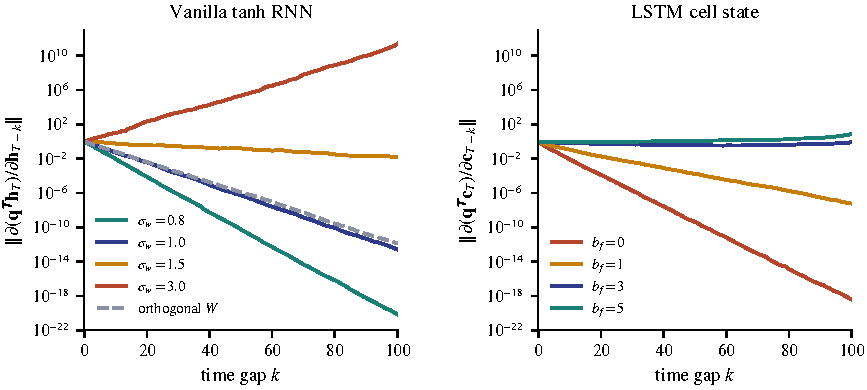
\includegraphics[width=\linewidth]{figures/n14_gradnorm.pdf}
\caption{Norm of the gradient that a unit probe vector $\vect{q}$ applied to the state at time $T$ sends back $k$ steps,
at initialisation (median of 20 random networks, $d = 64$, inputs $\pm 1$ at random). Left: tanh RNNs with Gaussian
recurrent weights $W_{ij} \sim \Normal(0, \sigma_w^2/d)$, whose spectral radius is close to $\sigma_w$, and with an orthogonal $W$; the
state is $\hv$. At $k = 100$ the norm is $7 \times 10^{-21}$ for $\sigma_w = 0.8$, $3 \times 10^{-13}$ for $\sigma_w = 1$, $0.018$ for
$\sigma_w = 1.5$ and $2 \times 10^{11}$ for $\sigma_w = 3$; orthogonal weights give $1 \times 10^{-12}$. Right: LSTMs
(Section~\ref{sec:lstm}) with recurrent weights $\Normal(0, 1/d)$ for every gate ($\sigma_w = 1$), input weights $\Normal(0, 1)$
and forget-gate bias $b_f$; the state is the cell $\cv$, and all paths are included. At $k = 100$: $4 \times 10^{-19}$,
$6 \times 10^{-8}$, $0.8$ and $7$ for $b_f = 0, 1, 3, 5$. Colours are not matched between the panels.}
\label{fig:gradnorm}
\end{figure}

Figure~\ref{fig:gradnorm} (left) measures these products in random tanh networks whose recurrent weights are drawn as
$W_{ij} \sim \Normal(0, \sigma_w^2/d)$; the \emph{gain} $\sigma_w$ (the $\sigma_w$ of the physics box of Note~12, Section~7) then sets the spectral radius, $\rho(W) \approx \sigma_w$. Each curve is
close to a straight line on the logarithmic axis: the gradient changes by a roughly constant factor per step, as
\eqref{eq:bound} suggests. For small gains it vanishes; for $\sigma_w = 3$ it explodes by eleven orders of magnitude over a
hundred steps. Even at $\sigma_w = 1$ it vanishes, because the inputs and the state keep units away from zero, where the
derivatives in $D_s$ are below one, so every factor shrinks a little; the gain must be raised to about $1.5$ before the
decay becomes slow, and there the network is close to the boundary between order and chaos (box below). An orthogonal
$W$, whose singular values are all one, still vanishes, because the factors $D_s$ have entries below one whenever units
are away from zero.

\paragraph{Consequences} Exploding gradients are spectacular: the loss jumps, parameters fly off, and training may
produce overflow. Vanishing gradients are silent but worse. The gradient of $W$ in \eqref{eq:bpttgrads} is a sum of
terms from all gaps $k$, and the terms with large $k$ are exponentially smaller than those with small $k$; the gradient is
dominated by short-range dependencies, and a dependency spanning fifty steps --- the subject of a sentence that decides
the form of a verb many words later, or a slow drift in a sensor --- produces a signal buried under the short-range ones.
Bengio, Simard and Frasconi showed that this is a structural dilemma: a recurrent network that stores information
robustly, against small perturbations of its state, operates in a regime where the gradient with respect to the past
vanishes~\cite{bengio1994}.

\begin{figure}[htbp]
\centering
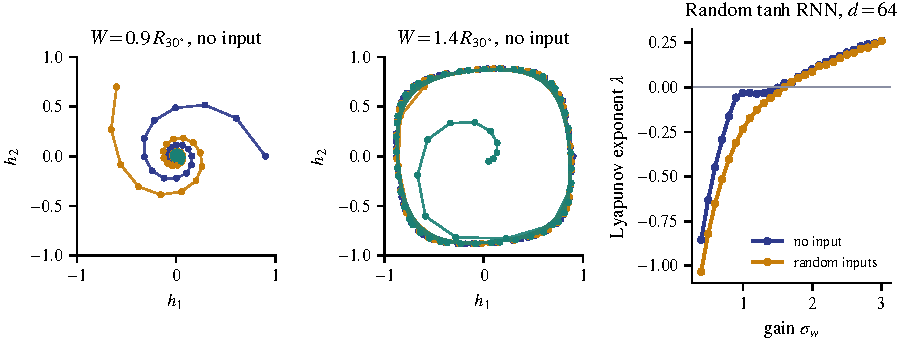
\includegraphics[width=\linewidth]{figures/n14_dynamics.pdf}
\caption{A recurrent network as a dynamical system. Left and centre: trajectories of a two-unit network
$\hv_t = \tanh(W\hv_{t-1})$ with $W$ a rotation by $30^\circ$ scaled by $0.9$ or $1.4$, from three starting points. With
$0.9$ every trajectory spirals into the stable fixed point $\vect{0}$; with $1.4$ the origin is unstable and all
trajectories settle on the same attracting closed curve, the discrete-time counterpart of a \emph{limit cycle}. Right:
largest Lyapunov exponent $\lambda$ of random tanh networks ($d = 64$, mean of five networks) against the gain $\sigma_w$, without
input and with the random inputs of Figure~\ref{fig:gradnorm}. With inputs, $\lambda = -0.40$ at $\sigma_w = 0.8$, $-0.23$ at
$\sigma_w = 1$ and $+0.26$ at $\sigma_w = 3$, comparable to the average per-step slopes of $\ln\norm{\cdot}$ in
Figure~\ref{fig:gradnorm} ($-0.47$, $-0.29$ and $+0.26$; on the base-10 axis of that figure, divide by
$\ln 10 \approx 2.30$). Both curves change sign near $\sigma_w \approx 1.6$.}
\label{fig:dynamics}
\end{figure}

\begin{physics}{Lyapunov exponents: vanishing and exploding gradients in time}
For a dynamical system $\hv_t = F(\hv_{t-1})$, a small perturbation $\vect{\epsilon}_0$ of the initial state evolves as
$\vect{\epsilon}_k \approx \big(\prod_s J_s\big)\vect{\epsilon}_0$, with $J_s$ the Jacobian along the trajectory --- the
same product as \eqref{eq:jacprod}. Its typical growth rate, $\lambda = \lim_{k\to\infty}\frac1k\ln\norm{\vect{\epsilon}_k}$,
is the largest \emph{Lyapunov exponent}. Numerically, one propagates a tangent vector, $\vect{\epsilon} \gets J_s\vect{\epsilon}$,
renormalises it to unit length after each step, and averages the logarithms of the growth factors. A negative exponent
means that the system forgets its initial condition and settles onto a stable fixed point (Figure~\ref{fig:dynamics},
left, where $\lambda = \ln 0.9 = -0.105$); on an attracting closed curve (centre) the largest exponent is zero, because
displacements along the curve neither grow nor shrink; a positive exponent means chaos, with nearby trajectories
separating as $e^{\lambda k}$, and $1/\lambda$ is then the \emph{Lyapunov time}, over which a small error grows by a
factor $e$. Backpropagation applies the transposed Jacobians to a gradient, and transposition does not change the
asymptotic growth rate, so \emph{vanishing gradients are a negative Lyapunov exponent and exploding gradients a positive
one}: $\norm{\partial\ell_T/\partial\hv_{T-k}} \sim e^{\lambda k}$. Figure~\ref{fig:dynamics} (right) measures $\lambda$ for
random tanh networks; the measured exponents are comparable to the natural-log slopes of Figure~\ref{fig:gradnorm}. For
large continuous-time random networks Sompolinsky, Crisanti and Sommers found a sharp transition to chaos at gain
$\sigma_w = 1$~\cite{sompolinsky1988}, and a driving input suppresses chaos~\cite{rajan2010}: in the right panel the input
lowers $\lambda$ strongly below the transition ($-0.235$ against $-0.032$ at $\sigma_w = 1$). In these small networks
($d = 64$) both curves cross zero only near $\sigma_w \approx 1.6$, and the input-free curve stays close to zero between $\sigma_w = 1$
and $1.5$. The depth version of this order--chaos transition is the physics box of Note~12, Section~7; initialising
near $\lambda = 0$ is the recurrent counterpart of its critical initialisation.
\end{physics}

\subsection{First remedies: clipping and orthogonal initialisation}\label{sec:remedies}

\paragraph{Gradient clipping} Explosion is handled by gradient clipping (Note~7, Section~7;
Algorithm~\ref{alg:tbptt})~\cite{pascanu2013}, standard in most recurrent and transformer training recipes. The picture
behind it is a loss surface with steep ``cliffs'' --- regions where a small change of $W$ crosses a \emph{bifurcation}, a
qualitative change of the dynamics such as a fixed point turning unstable (Figure~\ref{fig:dynamics}, left versus
centre) --- on which an unclipped step would throw the parameters far away. It does nothing for vanishing gradients.

\paragraph{Orthogonal initialisation} An orthogonal matrix, $Q\T Q = QQ\T = I$, preserves norms:
$\norm{Q\vect{u}}^2 = \vect{u}\T Q\T Q\vect{u} = \norm{\vect{u}}^2$, and so does its transpose. All its eigenvalues have
modulus one and all its singular values equal one. Initialising $W$ as a random orthogonal matrix therefore makes the
linear part of every factor in \eqref{eq:jacprod} norm-preserving, so that at initialisation the products neither
grow nor shrink because of $W$; deviations come only from the derivatives $D_s$, which are close to $I$ while the units
are near zero~\cite{saxe2014}. For example, the rotation by $60^\circ$ maps $(3, 4)$ to $(-1.964, 4.598)$, again of norm
$5$, and its powers never change the norm. A related recipe for ReLU recurrent networks (IRNN) initialises $W = I$ and the
biases to zero, so that the state is copied unchanged until learning modifies it~\cite{le2015}. Both are good starts, but
neither survives training automatically, and Figure~\ref{fig:gradnorm} shows that with saturating units an orthogonal $W$
still lets the gradient vanish. The durable fix is architectural.

\begin{algorithm}[htbp]
\caption{Random orthogonal initialisation of a recurrent matrix}\label{alg:orth}
\begin{algorithmic}[1]
\Require size $d$; gain $\sigma_w$ (usually $1$)
\Function{OrthogonalInit}{$d, \sigma_w$}
  \State draw $A \in \R^{d \times d}$ with independent $\Normal(0, 1)$ entries
  \State $Q, R \gets \mathrm{QR}(A)$ \Comment{Gram--Schmidt or Householder, $O(d^3)$}
  \State $Q \gets Q\,\diag(\mathrm{sign}(R_{11}), \dots, \mathrm{sign}(R_{dd}))$ \Comment{makes $Q$ uniformly distributed}
  \State \Return $W = \sigma_w\,Q$
\EndFunction
\end{algorithmic}
\end{algorithm}

\begin{runtime}{orthogonal initialisation}
\emph{Time}: $O(d^3)$ for the QR factorisation, once before training; $d = 1024$ takes about $10^9$ operations, a fraction of
a second. \emph{Memory}: $O(d^2)$, the size of $W$ itself. No cost during training or prediction. Without the sign correction
the distribution of $Q$ depends on the convention of the QR routine; with it, $Q$ is uniformly (Haar) distributed over the
orthogonal group.
\end{runtime}

\needspace{8\baselineskip}
\section{Long short-term memory}\label{sec:lstm}

The \emph{long short-term memory} (LSTM) of Hochreiter and Schmidhuber~\cite{hochreiter1997}, in the form with a forget
gate introduced by Gers, Schmidhuber and Cummins~\cite{gers2000}, adds to the hidden state $\hv_t$ a second state, the
\emph{cell} $\cv_t \in \R^d$, which is updated \emph{additively} and read and written through multiplicative \emph{gates}.
Each gate is a vector of numbers between $0$ and $1$ computed from the current input and the previous hidden state:
\begin{equation}\label{eq:gates}
\begin{aligned}
  \iv_t &= \sigma\big(W_i\hv_{t-1} + U_i\x_t + \bv_i\big) && \text{input gate: how much new content to write,} \\
  \fv_t &= \sigma\big(W_f\hv_{t-1} + U_f\x_t + \bv_f\big) && \text{forget gate: how much of the old cell to keep,} \\
  \ov_t &= \sigma\big(W_o\hv_{t-1} + U_o\x_t + \bv_o\big) && \text{output gate: how much of the cell to expose,}
\end{aligned}
\end{equation}
with the logistic sigmoid $\sigma$ (Note~11, Section~2). The cell and the hidden state are then updated as
\begin{equation}\label{eq:cell}
  \ctil_t = \tanh\big(W_c\hv_{t-1} + U_c\x_t + \bv_c\big), \qquad
  \cv_t = \fv_t \odot \cv_{t-1} + \iv_t \odot \ctil_t, \qquad
  \hv_t = \ov_t \odot \tanh(\cv_t) .
\end{equation}
The candidate $\ctil_t$ is what a plain RNN would compute. The cell keeps a gated fraction of its old content and adds a
gated fraction of the candidate; the hidden state, which feeds the output and the gates of the next step, is a gated,
squashed view of the cell. The gates are soft switches: with $\fv_t = \vect{1}$, $\iv_t = \vect{0}$ the cell is copied
unchanged, with $\fv_t = \vect{0}$ it is erased, and every value in between is possible and differentiable.

\needspace{8\baselineskip}
\begin{worked}{6. One LSTM step by hand}
Take one unit ($d = e = 1$), previous state $h_{t-1} = 0.5$, previous cell $c_{t-1} = 1$, input $x_t = 1$, all biases zero
and the weights $(W_i, U_i) = (-2, 1)$, $(W_f, U_f) = (2, 1)$, $(W_o, U_o) = (2, -1)$, $(W_c, U_c) = (0, 1)$. The
pre-activations are
\[
  a_i = -2(0.5) + 1 = 0, \quad a_f = 2(0.5) + 1 = 2, \quad a_o = 2(0.5) - 1 = 0, \quad a_c = 0 + 1 = 1 ,
\]
so $i_t = \sigma(0) = 0.5$, $f_t = \sigma(2) = 0.881$, $o_t = 0.5$ and $\tilde c_t = \tanh 1 = 0.762$. Then
\[
  c_t = 0.881 \times 1 + 0.5 \times 0.762 = 0.881 + 0.381 = 1.262, \qquad h_t = 0.5\tanh(1.262) = 0.5 \times 0.852 = 0.426 .
\]
The cell has grown beyond $1$, which a tanh unit could never do: it is not squashed, only the read-out is. Along the
direct path, $\partial c_t/\partial c_{t-1} = f_t = 0.881$ --- no weight and no tanh derivative appear in this factor.
\end{worked}

\paragraph{Derivation: why the additive cell helps} Differentiate \eqref{eq:cell} with respect to the previous cell. The
cell enters $\cv_t$ directly through $\fv_t \odot \cv_{t-1}$, and indirectly through $\hv_{t-1} = \ov_{t-1} \odot \tanh(
\cv_{t-1})$, on which all gates and the candidate of step $t$ depend:
\begin{equation}\label{eq:celljac}
  \frac{\partial \cv_t}{\partial \cv_{t-1}} = \diag(\fv_t) + \sum_{q \in \{i, f, c\}}
  \frac{\partial \cv_t}{\partial \av^{(q)}_t}\, W_q\, \diag\big(\ov_{t-1} \odot (1 - \tanh^2\cv_{t-1})\big) ,
\end{equation}
where $\av^{(q)}_t$ is the pre-activation of gate $q$ (or of the candidate). These factors are diagonal: with
$\sigma' = \sigma(1 - \sigma)$ (Note~11, Section~2),
\[
  \frac{\partial\cv_t}{\partial\av^{(i)}_t} = \diag\big(\ctil_t \odot \iv_t \odot (1 - \iv_t)\big), \quad
  \frac{\partial\cv_t}{\partial\av^{(f)}_t} = \diag\big(\cv_{t-1} \odot \fv_t \odot (1 - \fv_t)\big), \quad
  \frac{\partial\cv_t}{\partial\av^{(c)}_t} = \diag\big(\iv_t \odot (1 - \ctil_t^2)\big) .
\]
The first term of \eqref{eq:celljac} is the new element. Keeping
only it along a path of $k$ steps,
\[
  \frac{\partial \cv_T}{\partial \cv_{T-k}}\bigg|_{\text{direct}} = \diag\big(\fv_T \odot \fv_{T-1} \odot \cdots \odot \fv_{T-k+1}\big) :
\]
no recurrent matrix and no derivative of a squashing function, only the forget gates. If the network keeps its forget
gates near one for a unit, error flows back along that unit's cell for as long as the gate stays open --- Hochreiter and
Schmidhuber's ``constant error carousel''. Unrolling the update shows the same thing in the forward direction:
\[
  \cv_t = \sum_{t' \le t} \big(\fv_t \odot \cdots \odot \fv_{t'+1}\big) \odot \iv_{t'} \odot \ctil_{t'}
  \qquad (\text{with } \cv_0 = \vect{0}),
\]
a sum of everything ever written, each entry discounted by the forget gates passed since. The network \emph{learns},
through the gates, when to remember and when to forget, and the gradient no longer has to fight a fixed contraction
factor. The indirect terms of \eqref{eq:celljac} still contain $W$ and can still vanish or explode, which is why clipping
remains useful.

\paragraph{Forget-gate bias} At initialisation the gate pre-activations are near zero, so $\fv_t \approx \sigma(\bv_f)$.
With $\bv_f = \vect{0}$ every forget gate is about $\frac12$ and the direct path decays like $2^{-k}$, no better than a poorly
scaled plain RNN. Initialising $\bv_f$ to $1$ or more makes the network remember by default and learn to forget, rather
than the reverse; Jozefowicz, Zaremba and Sutskever found that a bias of $1$ markedly improves LSTMs on several
tasks~\cite{jozefowicz2015}. With the gate held at $\sigma(b_f)$ the direct path after $k = 20$ steps is
\[
  \sigma(b_f)^{20} = 9.5 \times 10^{-7},\ \ 1.9 \times 10^{-3},\ \ 0.38,\ \ 0.87 \qquad\text{for } b_f = 0, 1, 3, 5 .
\]
Figure~\ref{fig:gradnorm} (right) shows the full gradient, all paths included, in random LSTMs: with $b_f = 0$ it vanishes
like a plain RNN, with $b_f = 3$ it stays of order one for a hundred steps. The full gradient exceeds the direct-path
product ($\sigma(3)^{100} = 0.008$) because the indirect terms of \eqref{eq:celljac}, which contain the matrices $W_q$,
add to it; for $b_f = 5$ they even make it grow slowly ($7$ at $k = 100$).

\begin{physics}{the cell is a leaky integrator with a learned time constant}
With a constant forget gate $f$ and input $u_t = i_t\tilde c_t$, the cell obeys $c_t = f c_{t-1} + u_t$. The Euler step
(step $1$) of $\tau\dot c = -c + \tau u(t)$ has this form with $f = 1 - 1/\tau$: an RC circuit, a low-pass filter, a damped
mode. Matching the decay of the impulse response exactly, $f^k = e^{-k/\tau}$, gives the time constant
\[
  \tau = -\frac{1}{\ln f} \approx \frac{1}{1 - f} \quad (f \to 1) ,
\]
so $f = 0.5$, $0.9$ and $0.99$ give memories of about $1.4$, $9.5$ and $99.5$ steps. The forget-gate biases $b_f = 0, 1, 3, 5$ of
the previous paragraph correspond to $\tau = 1.4$, $3.2$, $21$ and $149$ steps. An LSTM is thus a bank of leaky integrators
whose time constants are not fixed but set at every step by a learned function of the input and the state: a unit
can hold a value for hundreds of steps and then reset it in one. Physicists who model a detector pulse or a slowly
varying background with a filter of chosen time constant will recognise the structure; the LSTM chooses its own.
\end{physics}

\paragraph{Variants} Many modifications have been tried. \emph{Peephole connections} let the gates see the cell itself,
adding terms $\vect{p}_q \odot \cv_{t-1}$ (or $\cv_t$ for the output gate) to the gate pre-activations~\cite{gers2000peep}.
\emph{Coupled} input and forget gates set $\iv_t = \vect{1} - \fv_t$, so that writing and forgetting are tied. A large
empirical study of eight variants on speech, handwriting and music found none clearly better than the standard LSTM; the
forget gate and the squashing of the output were the most important components, while coupling the gates or removing
the peepholes did not hurt~\cite{greff2017}.

\section{Gated recurrent units}\label{sec:gru}

The \emph{gated recurrent unit} (GRU) of Cho et al.~\cite{cho2014} keeps the additive update of the LSTM with fewer
parts: no separate cell, two gates instead of three.
\begin{equation}\label{eq:gru}
\begin{aligned}
  \zv_t &= \sigma\big(W_z\hv_{t-1} + U_z\x_t + \bv_z\big), \qquad
  \rv_t = \sigma\big(W_r\hv_{t-1} + U_r\x_t + \bv_r\big), \\
  \htil_t &= \tanh\big(W_h(\rv_t \odot \hv_{t-1}) + U_h\x_t + \bv_h\big), \qquad
  \hv_t = (\vect{1} - \zv_t) \odot \hv_{t-1} + \zv_t \odot \htil_t .
\end{aligned}
\end{equation}
The \emph{update gate} $\zv_t$ plays the roles of both the input gate and the forget gate of the LSTM, coupled as
$\iv = \zv$, $\fv = \vect{1} - \zv$: the new state is a convex combination of the old state and the candidate, so it stays
inside $[-1, 1]^d$. The \emph{reset gate} $\rv_t$ decides how much of the old state the candidate may use; with
$\rv_t = \vect{0}$ the candidate is computed from the input alone, as if the sequence had just started. The state is
exposed directly, without an output gate. Along the direct path, $\partial\hv_t/\partial\hv_{t-1}$ contains the term $\diag(\vect{1} - \zv_t)$,
the counterpart of $\diag(\fv_t)$ in \eqref{eq:celljac}. Here $\zv_t$ is the update gate, not the logits of
\eqref{eq:rnn}. Conventions differ: Cho et al.\ and PyTorch write $\zv_t \odot \hv_{t-1} + (1 - \zv_t)\odot\htil_t$, so
their $\zv_t$ is the fraction kept rather than the fraction written, and some libraries apply the reset gate after the product, $\rv_t \odot
(W_h\hv_{t-1})$. The behaviour is similar.

\begin{algorithm}[htbp]
\caption{One step of an LSTM and of a GRU (the affine maps of all gates are one matrix product)}\label{alg:lstm}
\begin{algorithmic}[1]
\Require previous $\hv_{t-1}$ (and $\cv_{t-1}$ for the LSTM); input $\x_t$; stacked weights
  $W_\star \in \R^{4d \times d}$, $U_\star \in \R^{4d \times e}$, $\bv_\star \in \R^{4d}$ (LSTM) or $3d$ rows (GRU)
\Function{LSTMStep}{$\hv_{t-1}, \cv_{t-1}, \x_t$}
  \State $[\av^{(i)}; \av^{(f)}; \av^{(o)}; \av^{(c)}] \gets W_\star\hv_{t-1} + U_\star\x_t + \bv_\star$
    \Comment{$O(4d(d + e))$, the whole cost}
  \State $\iv \gets \sigma(\av^{(i)})$; \ $\fv \gets \sigma(\av^{(f)})$; \ $\ov \gets \sigma(\av^{(o)})$; \ $\ctil \gets \tanh(\av^{(c)})$
  \State $\cv_t \gets \fv \odot \cv_{t-1} + \iv \odot \ctil$; \ $\hv_t \gets \ov \odot \tanh(\cv_t)$ \Comment{$O(d)$}
  \State \Return $\hv_t, \cv_t$
\EndFunction
\Function{GRUStep}{$\hv_{t-1}, \x_t$}
  \State $[\av^{(z)}; \av^{(r)}] \gets W_{zr}\hv_{t-1} + U_{zr}\x_t + \bv_{zr}$; \ $\zv \gets \sigma(\av^{(z)})$; \ $\rv \gets \sigma(\av^{(r)})$
  \State $\htil \gets \tanh\big(W_h(\rv \odot \hv_{t-1}) + U_h\x_t + \bv_h\big)$ \Comment{reset gate acts before $W_h$}
  \State \Return $\hv_t = (1 - \zv) \odot \hv_{t-1} + \zv \odot \htil$
\EndFunction
\end{algorithmic}
\end{algorithm}

\begin{runtime}{LSTM and GRU cells}
\emph{Time}: $O(4d(d + e))$ multiply--adds per step for the LSTM and $O(3d(d + e))$ for the GRU, against $O(d(d + e))$ for a
plain RNN; the element-wise operations are $O(d)$. A sequence costs $T$ times as much, and BPTT through the cell (by
automatic differentiation) about twice the forward pass. \emph{Memory}: $4d(d + e + 1)$ parameters for the LSTM and
$3d(d + e + 1)$ for the GRU (libraries that keep two bias vectors per gate add $4d$ or $3d$); during training about six
vectors of size $d$ per step (gates, candidate, cell, state) must be stored. \emph{Generation}: $O(4d(d + e))$ per token and a
state of $2d$ numbers.
\end{runtime}

\begin{worked}{7. Counting parameters of recurrent cells}
For hidden size $d = 512$ and input size $e = 256$, the cells have
\[
  \text{plain RNN: } 393\,728 \ (\text{Section~\ref{sec:deep}}), \qquad \text{GRU: } 3d(d + e + 1) = 1\,181\,184, \qquad
  \text{LSTM: } 1\,574\,912
\]
parameters, the last being $4d(d + e + 1)$; the forward cost per step is in the same ratio $1 : 3 : 4$. At equal parameter budget a GRU can therefore be
about $15\%$ wider than an LSTM ($\sqrt{4/3} \approx 1.15$ when $d \gg e$). Which is better depends on the task; with
the forget-gate bias of Section~\ref{sec:lstm}, comparisons generally find the two close.
\end{worked}

\begin{modern}{where gated recurrent networks are still used}
Transformers (Note~15) have replaced recurrent networks in most of language processing, but gated RNNs remain a strong
and economical choice wherever data arrive as a stream and the model must run with constant memory per step. In
probabilistic forecasting, DeepAR trains one autoregressive LSTM on many related time series (the demand for thousands of
products, for instance) and outputs a predictive distribution for each future value rather than a point
forecast~\cite{salinas2020}. Small LSTMs and GRUs run on devices with tight memory, in streaming speech and sensor
processing, and in control. Google's neural machine-translation system, deployed in 2016, was a stack of eight LSTM layers in the
encoder and eight in the decoder, with residual connections and attention~\cite{wu2016} --- one of the last large
recurrent systems before the transformer, and, with its attention, a bridge to Note~15.
\end{modern}

\section{Sequence-to-sequence learning}\label{sec:seq2seq}

Many tasks map one sequence to another of different length with no position-by-position alignment: translating a
sentence, summarising a document, transcribing speech, turning a question into an answer. The output sequence
$w_{1:T'} = (w_1, \dots, w_{T'})$ cannot be predicted one label per input position, so the model is a \emph{conditional} language
model:
\begin{equation}\label{eq:condlm}
  p(w_1, \dots, w_{T'} \mid \x_1, \dots, \x_{T}) = \prod_{t=1}^{T'} p(w_t \mid w_{<t}, \x_{1:T}) .
\end{equation}
The \emph{encoder--decoder} architecture~\cite{cho2014,sutskever2014} uses two recurrent networks. The \emph{encoder}
reads the input sequence and its final state becomes a fixed-size summary $\vect{s} = \hv^{\mathrm{enc}}_T$, the
\emph{context vector}. The \emph{decoder} is an RNN language model whose initial state is $\vect{s}$ (or which receives
$\vect{s}$ as an extra input at every step); it starts from \bos\ and produces the output tokens one by one until \eos.
Figure~\ref{fig:seq2seq} draws the arrangement. Several details were found to matter:
\begin{itemize}
\item the encoder and the decoder have \emph{separate} parameters (they read different languages and do different jobs);
\item stacking several LSTM layers in both helps substantially;
\item Sutskever, Vinyals and Le found that reading the source sentence \emph{in reverse order} improved their LSTM
  translation model markedly~\cite{sutskever2014}: the first source words then sit close to the first target words in the
  unrolled graph, which shortens the paths the gradient must travel at the beginning of the output.
\end{itemize}

\begin{figure}[htbp]
\centering
\begin{tikzpicture}[>=Stealth, enc/.style={draw=teal, fill=teal!8, rounded corners=2pt, minimum width=8mm,
  minimum height=6mm, font=\small}, dec/.style={draw=indigo, fill=indigo!6, rounded corners=2pt, minimum width=8mm,
  minimum height=6mm, font=\small}, io/.style={font=\small}]
  \foreach \t/\xx/\w in {1/0/{\x_1}, 2/1.4/{\x_2}, 3/2.8/{\x_3}, 4/4.2/{\x_4}} {
    \node[enc] (e\t) at (\xx,0) {};
    \node[io] (ex\t) at (\xx,-1.1) {$\w$};
    \draw[->] (ex\t) -- (e\t);
  }
  \draw[->] (e1) -- (e2); \draw[->] (e2) -- (e3); \draw[->] (e3) -- (e4);
  \foreach \t/\xx/\inp/\out in {1/6.7/\bos/{w_1}, 2/8.1/{w_1}/{w_2}, 3/9.5/{w_2}/{w_3}, 4/10.9/{w_3}/\eos} {
    \node[dec] (d\t) at (\xx,0) {};
    \node[io] (dx\t) at (\xx,-1.1) {$\inp$};
    \node[io] (dy\t) at (\xx,1.15) {$\out$};
    \draw[->] (dx\t) -- (d\t);
    \draw[->] (d\t) -- (dy\t);
  }
  \draw[->] (d1) -- (d2); \draw[->] (d2) -- (d3); \draw[->] (d3) -- (d4);
  \draw[->, very thick, amber] (e4) -- node[above, font=\scriptsize, text=amber] {$\vect{s} = \hv^{\mathrm{enc}}_4$} (d1);
  \draw[->, densely dotted, mute] (dy1.east) to[out=-10, in=135] (dx2.north west);
  \draw[->, densely dotted, mute] (dy2.east) to[out=-10, in=135] (dx3.north west);
  \draw[->, densely dotted, mute] (dy3.east) to[out=-10, in=135] (dx4.north west);
  \node[font=\scriptsize, text=teal] at (2.1,0.65) {encoder};
  \node[font=\scriptsize, text=indigo] at (8.8,-1.75) {decoder: a conditional language model};
\end{tikzpicture}
\caption{An encoder--decoder. The encoder (teal) reads the source $\x_1, \dots, \x_4$; its final state $\vect{s}$ is the only
information about the source that reaches the decoder (indigo). The decoder's input at each step is the previous target
token: the true one during training (teacher forcing), its own previous output at test time (dotted arrows).}
\label{fig:seq2seq}
\end{figure}

\paragraph{Training with teacher forcing} The loss is the negative log of \eqref{eq:condlm} for the reference output,
summed over the training pairs. During training the decoder receives the \emph{true} previous token $w_{t-1}$ as input,
not its own prediction: \emph{teacher forcing}. The loss then decomposes into $T'$ next-token cross-entropies that are all
computed in one forward pass, and the gradient flows through decoder and encoder alike by BPTT. Sequences in a mini-batch
have different lengths; they are padded to a common length with a padding token whose positions are excluded from the
loss by a \emph{mask}, and grouping sequences of similar length into the same mini-batch (\emph{bucketing}) keeps the
wasted computation small.

\paragraph{Exposure bias} At test time the true previous token is not available, and the decoder must consume its own
outputs. It has never been trained on prefixes containing its own mistakes, so an early error can lead it into
unfamiliar states where it makes more errors. This mismatch between training and use is called \emph{exposure bias}.
\emph{Scheduled sampling} replaces, with a probability that increases during training, the true previous token by a token
sampled from the model~\cite{bengio2015}; in practice teacher forcing remains the standard, because it is simple and
stable and gives every target token's loss in one decoder pass (parallel over positions only for the attention-based
decoders of Note~15; a recurrent decoder still loops over $t$).

\begin{algorithm}[htbp]
\caption{One training step of an encoder--decoder with teacher forcing}\label{alg:seq2seq}
\begin{algorithmic}[1]
\Require mini-batch of pairs $(\x^{(m)}_{1:T_m}, w^{(m)}_{1:T'_m})$, each $w^{(m)}$ ending with \eos; encoder and decoder
  RNNs; output layer; optimiser
\Function{Seq2SeqStep}{batch}
  \State pad sources and targets to the longest lengths in the batch
  \State masks: $\mu^{(m)}_t = 1$ for real target tokens, $0$ for padding
  \For{each pair $m$ (in parallel)}
    \State $\vect{s} \gets$ final state of the encoder on $\x^{(m)}$ \Comment{Algorithm~\ref{alg:rnnfwd} without outputs}
    \State $\hv \gets \vect{s}$; \ $w^{(m)}_0 \gets \bos$; \ $\ell^{(m)} \gets 0$
    \For{$t = 1, \dots, T'_{\max}$}
      \State $\hv \gets \textsc{DecoderStep}(\hv, \ev(w^{(m)}_{t-1}))$ \Comment{true previous token: teacher forcing}
      \State $\ell^{(m)} \gets \ell^{(m)} - \mu^{(m)}_t\log\softmax(V_{\mathrm{out}}\hv + \bv_y)_{w^{(m)}_t}$
    \EndFor
  \EndFor
  \State $J \gets \sum_m \ell^{(m)} \big/ \sum_{m,t}\mu^{(m)}_t$ \Comment{mean loss per real target token}
  \State BPTT through decoder and encoder; clip the gradient; optimiser step
\EndFunction
\end{algorithmic}
\end{algorithm}

\begin{runtime}{encoder--decoder training}
\emph{Time} per pair: $O\big(T\,c_{\mathrm{cell}} + T'(c_{\mathrm{cell}} + dV)\big)$ forward, with $c_{\mathrm{cell}} = 4Ld(d + e)$
for an $L$-layer LSTM; backward about twice that. \emph{Memory}: $O((T + T')Ld)$ stored states per pair. \emph{Padding}
wastes the fraction of masked positions; bucketing by length keeps it small. Teacher forcing lets all $T'$ output
losses be computed in one pass of the decoder; the encoder and decoder loops themselves remain sequential in time.
\end{runtime}

\begin{worked}{8. Where the parameters of a translation model are}
Sutskever, Vinyals and Le used four LSTM layers with $d = 1000$ cells in both encoder and decoder, word embeddings of size
$e = 1000$, a source vocabulary of $160\,000$ words and a target vocabulary of $80\,000$ words~\cite{sutskever2014}. Count:
\begin{itemize}
\item embeddings: $(160\,000 + 80\,000) \times 1000 = 240\,000\,000$;
\item LSTM layers: each has $4 \times 1000 \times (1000 + 1000 + 1) = 8\,004\,000$; eight layers give $64\,032\,000$;
\item output softmax: $80\,000 \times 1001 = 80\,080\,000$.
\end{itemize}
Total $384\,112\,000$, the $384$ million parameters the authors report. Five-sixths of them sit in the vocabulary
tables at the two ends; the recurrent layers that do the ``translating'' hold one-sixth. The whole meaning of a source
sentence, however long, must nevertheless pass through one context vector of $4 \times 2 \times 1000 = 8000$ numbers (the
states and cells of the four encoder layers).
\end{worked}

\paragraph{The bottleneck} Everything the decoder learns about the source must pass through the fixed-size vector
$\vect{s}$, whatever the length of the input. Letting the decoder consult all encoder states, with weights it computes
itself, removes this bottleneck: this is \emph{attention} (Note~15, Sections~1 and~2).

\section{Decoding: greedy search, beam search and sampling}\label{sec:decode}

Once trained, a conditional language model defines a distribution over output sequences. For translation or
transcription one wants the most probable output,
\begin{equation}\label{eq:map}
  \hat{w}_{1:T'} = \argmax_{w_{1:T'}} \sum_{t=1}^{T'} \log p(w_t \mid w_{<t}, \x) ,
\end{equation}
but the number of candidates is $V^{T'}$, and the network's state after a prefix depends on the whole prefix, so dynamic
programming does not apply. Exact search is out of reach; decoders approximate it.

\paragraph{Greedy decoding} Take the most probable token at every step and feed it back. This costs one decoder step per
token but can be badly wrong: a token that looks best now may lead only to poor continuations.

\paragraph{Beam search} Keep the $B$ best partial outputs (\emph{hypotheses}), ranked by their log-probability so far. At
each step, extend every hypothesis by every token, score the $BV$ extensions, and keep the best $B$. A hypothesis that
ends with \eos\ is complete and keeps its score; the search stops when the $B$ best hypotheses are all complete or a
maximum length is reached, and returns the best complete one. With $B = 1$ beam search is greedy decoding; with $B = V^{T'}$
it would be exhaustive. Small beams (a handful of hypotheses) were enough for most of the gain in
translation~\cite{sutskever2014}. Because every token multiplies the probability by a number below one, scores favour
short outputs; the usual correction ranks complete hypotheses by their log-probability divided by their length (or by a
power of it).

\begin{worked}{9. Greedy versus beam search on a tiny vocabulary}
The vocabulary is $\{a, b, \eos\}$ and outputs have at most two words before \eos\ (after two words, \eos\ is certain). The
decoder's distributions are
\begin{center}\small
\begin{tabular}{@{}lccc@{}}
\toprule
 & $a$ & $b$ & \eos \\
\midrule
$p(w_1)$ & $0.5$ & $0.4$ & $0.1$ \\
$p(w_2 \mid w_1 = a)$ & $0.3$ & $0.3$ & $0.4$ \\
$p(w_2 \mid w_1 = b)$ & $0.1$ & $0.1$ & $0.8$ \\
\bottomrule
\end{tabular}
\end{center}
\emph{Greedy}: $a$ (0.5), then \eos\ (0.4): output ``$a$'' with probability $0.5 \times 0.4 = 0.20$.
\emph{Beam, $B = 2$}: step~1 keeps $a$ ($\log 0.5 = -0.693$) and $b$ ($-0.916$); the complete hypothesis ``\eos'' ($0.1$) falls
out. Step~2 scores the six extensions:
\[
  aa\ 0.15,\quad ab\ 0.15,\quad a\,\eos\ 0.20,\quad ba\ 0.04,\quad bb\ 0.04,\quad b\,\eos\ 0.32 .
\]
The best two are $b\,\eos$ ($\log 0.32 = -1.139$) and $a\,\eos$ ($-1.609$), both complete, so the search stops and returns
``$b$'' with probability $0.32$. Enumerating all seven possible outputs ($b$: $0.32$; $a$: $0.20$; $aa$, $ab$: $0.15$ each,
since \eos\ is then certain; the empty output: $0.10$; $ba$, $bb$: $0.04$ each) confirms that $b$ is the most probable: greedy
search was misled by the attractive first token. Here normalising by length (two tokens for $b\,\eos$ and $a\,\eos$, three
for $aa\,\eos$) does not change the ranking: $-0.570$ for $b\,\eos$ against $-0.632$ for $aa\,\eos$ and $-0.805$ for $a\,\eos$.
\end{worked}

\begin{algorithm}[htbp]
\caption{Beam search decoding}\label{alg:beam}
\begin{algorithmic}[1]
\Require decoder state $\hv_0$ (e.g.\ the encoder's context $\vect{s}$); beam width $B$; maximum length $T_{\max}$
\Function{BeamSearch}{$\hv_0$}
  \State $\mathcal{H} \gets \{(\text{prefix} = (\bos),\ \text{score} = 0,\ \text{state} = \hv_0)\}$; \ $\mathcal{C} \gets \emptyset$
    \Comment{live and complete hypotheses}
  \For{$t = 1, \dots, T_{\max}$}
    \State $\mathcal{N} \gets \emptyset$
    \For{each $(\pi, s, \hv) \in \mathcal{H}$}
      \State $\hv' \gets \textsc{DecoderStep}(\hv, \ev(\text{last token of } \pi))$ \Comment{$O(c_{\mathrm{cell}})$}
      \State $\vect{q} \gets \log\softmax(V_{\mathrm{out}}\hv' + \bv_y)$ \Comment{$O(dV)$}
      \State add $(\pi \cdot k,\ s + q_k,\ \hv')$ to $\mathcal{N}$ for every token $k$ \Comment{or only the top $B$ tokens}
    \EndFor
    \State $\mathcal{K} \gets$ the $B$ highest-scoring elements of $\mathcal{N} \cup \mathcal{C}$
    \State $\mathcal{C} \gets$ the elements of $\mathcal{K}$ ending in \eos; \ $\mathcal{H} \gets$ the others
    \If{$\mathcal{H} = \emptyset$} \textbf{break} \Comment{the $B$ best are all complete} \EndIf
  \EndFor
  \State \Return the best element of $\mathcal{C}$ (of $\mathcal{H}$ if $\mathcal{C} = \emptyset$) \Comment{score, or score per token}
\EndFunction
\end{algorithmic}
\end{algorithm}

\begin{runtime}{beam search}
\emph{Time}: $O\big(T_{\max}B(c_{\mathrm{cell}} + dV)\big)$ for the decoder steps and softmaxes, plus $O(T_{\max}BV)$ for
finding the best extensions (a partial selection, not a full sort, of the $BV$ candidates; taking each hypothesis's own
top $B$ tokens first, $O(V)$ each, leaves a final merge of only $B^2$ candidates). The cost is $B$ times that of greedy decoding, and
the $B$ hypotheses are processed as one mini-batch. \emph{Memory}: $B$ decoder states and $B$ prefixes, $O(B(Ld + T_{\max}))$.
Beam search is approximate and not even monotone in $B$: a larger beam usually, but not always, finds a higher-scoring
output, and in translation very large beams sometimes produce \emph{worse} outputs (too short or generic), a sign that the
model's most probable sequence is not always the best one.
\end{runtime}

\paragraph{Sampling} When many outputs are acceptable (a story, a dialogue reply), one samples instead of maximising,
by the ancestral sampling of Section~\ref{sec:rnn}. Three modifications reshape each next-token distribution before
the draw. The \emph{temperature} $T_{\mathrm{temp}}$ of Note~2, modern box of Section~2.2 (written with a
subscript here to keep $T$ for lengths), divides the logits, $p_k \mapsto p_k^{1/T_{\mathrm{temp}}}/\sum_j
p_j^{1/T_{\mathrm{temp}}}$: values below one sharpen the distribution, values above one flatten it. \emph{Top-$k$}
sampling keeps only the $k$ most probable tokens and renormalises. \emph{Nucleus} (top-$p$) sampling keeps the smallest
set of most probable tokens whose probabilities add up to at least $p$, and renormalises~\cite{holtzman2020}. For the
first-step distribution of Worked example~9, $(0.5, 0.4, 0.1)$: temperature $0.5$ gives $(0.595, 0.381, 0.024)$ and
temperature $2$ gives $(0.427, 0.382, 0.191)$; top-$2$ sampling and nucleus sampling with $p = 0.8$ both keep $\{a, b\}$ and
sample them with probabilities $(0.556, 0.444)$.

\begin{algorithm}[htbp]
\caption{Autoregressive generation with temperature, top-$k$ and nucleus sampling}\label{alg:sample}
\begin{algorithmic}[1]
\Require decoder state $\hv_0$; temperature $T_{\mathrm{temp}} > 0$; optional $k$ (top-$k$) or $p$ (nucleus); maximum
  length $T_{\max}$
\Function{Sample}{$\hv_0$}
  \State $\hv \gets \hv_0$; \ $w \gets \bos$; \ output $\gets$ empty list
  \For{$t = 1, \dots, T_{\max}$}
    \State $\hv \gets \textsc{DecoderStep}(\hv, \ev(w))$ \Comment{$O(c_{\mathrm{cell}})$}
    \State $\zv \gets (V_{\mathrm{out}}\hv + \bv_y)/T_{\mathrm{temp}}$ \Comment{$O(dV)$}
    \State \textbf{if} top-$k$: set all but the $k$ largest entries of $\zv$ to $-\infty$ \Comment{partial selection, $O(V)$}
    \State $\vect{\pi} \gets \softmax(\zv)$
    \State \textbf{if} nucleus: sort $\vect{\pi}$, keep the shortest prefix of mass $\ge p$, renormalise
      \Comment{$O(V\log V)$}
    \State draw $w \sim \vect{\pi}$; \ append $w$ to the output \Comment{Note~2, Section~2.2}
    \If{$w = \eos$} \textbf{break} \EndIf
  \EndFor
  \State \Return the output
\EndFunction
\end{algorithmic}
\end{algorithm}

\begin{runtime}{sampling}
\emph{Time}: $O\big(T'(c_{\mathrm{cell}} + dV)\big)$ for an output of $T'$ tokens: one decoder step and one softmax per
token, as for greedy decoding; top-$k$ adds $O(T'V)$ for the partial selection, nucleus sampling $O(T'V\log V)$ for the
sort (or less with a partial sort). \emph{Memory}: the current state, $O(Ld)$ numbers, plus the $T'$ output tokens.
The steps are strictly sequential, and independent samples can be drawn in parallel as a mini-batch.
\end{runtime}

\begin{modern}{decoding a large language model}
Beam search remains the decoder of choice when there is essentially one right answer --- translation, speech
recognition. For open-ended generation it fails in a characteristic way: the most probable continuations of a text are
bland and repetitive, and maximising probability drives a model into loops. Holtzman et al.\ documented this
degeneration and proposed nucleus sampling as the remedy~\cite{holtzman2020}: it cuts off the unreliable tail of the
distribution, whose many individually improbable tokens together carry much probability, while keeping the variety of
the head. All of these controls act only on the output distribution of one step, so they apply unchanged to recurrent and transformer decoders.
\end{modern}

\section{Sequence classification and bidirectional networks}\label{sec:bidir}

\paragraph{Sequence classification} When a whole sequence receives one label --- the sentiment of a review, the class of
an event recorded as a time series, the type of a particle from the sequence of its hits --- the network must turn a
variable-length sequence into a fixed-size vector and classify it. The simplest summary is the final state $\hv_T$, as
for the encoder of Section~\ref{sec:seq2seq}. Formally this is a sequence-to-sequence problem whose output has a single
token, the label, so the encoder of Section~\ref{sec:seq2seq} followed by a softmax is enough. The final state is biased towards the end of the sequence, and averaging or taking the element-wise
maximum of all states, $\frac1T\sum_t\hv_t$ or $\max_t\hv_t$, often works better for long inputs. A softmax layer
(Note~11, Section~5) on this summary gives the class probabilities, and BPTT distributes the gradient of the single loss
over all time steps.

\paragraph{Bidirectional RNNs} When the whole input is available before any output is needed --- tagging a sentence,
labelling the frames of a recording, encoding the source of a translation --- there is no reason to label position $t$
from positions $1, \dots, t$ alone (Section~\ref{sec:deep}): the word after an ambiguous word often decides its
meaning. A \emph{bidirectional} RNN~\cite{schuster1997} runs two independent RNNs, one forward over $\x_1, \dots, \x_T$ and one
backward over $\x_T, \dots, \x_1$, and represents position $t$ by the concatenation of their states:
\begin{equation}\label{eq:birnn}
  \overrightarrow{\hv}_t = \mathrm{cell}_{\rightarrow}\big(\overrightarrow{\hv}_{t-1}, \x_t\big), \qquad
  \overleftarrow{\hv}_t = \mathrm{cell}_{\leftarrow}\big(\overleftarrow{\hv}_{t+1}, \x_t\big), \qquad
  \hv_t = \big[\overrightarrow{\hv}_t; \overleftarrow{\hv}_t\big] \in \R^{2d} .
\end{equation}
Now $\hv_t$ depends on the entire sequence and is centred on position $t$. Bidirectional layers can be stacked (the input of
layer $l$ is the concatenated $\hv^{(l-1)}_t$), and deep bidirectional LSTMs were for several years widely used for
speech recognition~\cite{graves2013speech} and for tagging. They are unusable when the future is not available: a
language model that generates text, or any system that must answer before the input ends (streaming speech, on-line
triggers), must stay causal.

\begin{algorithm}[htbp]
\caption{A bidirectional RNN tagger: forward pass}\label{alg:birnn}
\begin{algorithmic}[1]
\Require inputs $\x_1, \dots, \x_T$; forward and backward cells (separate parameters); output layer for $K$ labels
\Function{BiRNNTag}{$\x_{1:T}$}
  \State $\overrightarrow{\hv}_0 \gets \vect{0}$; \ \textbf{for} $t = 1, \dots, T$: $\overrightarrow{\hv}_t \gets \mathrm{cell}_{\rightarrow}(\overrightarrow{\hv}_{t-1}, \x_t)$
  \State $\overleftarrow{\hv}_{T+1} \gets \vect{0}$; \ \textbf{for} $t = T, \dots, 1$: $\overleftarrow{\hv}_t \gets \mathrm{cell}_{\leftarrow}(\overleftarrow{\hv}_{t+1}, \x_t)$
    \Comment{independent of the first loop}
  \For{$t = 1, \dots, T$}
    \State $\yv_t \gets \softmax\big(V_{\mathrm{out}}[\overrightarrow{\hv}_t; \overleftarrow{\hv}_t] + \bv_y\big)$ \Comment{$O(2dK)$}
  \EndFor
  \State \Return $\yv_1, \dots, \yv_T$ \Comment{loss: $-\sum_t \log y_{t,\,y^\star_t}$, gradients by BPTT in both directions}
\EndFunction
\end{algorithmic}
\end{algorithm}

\begin{runtime}{bidirectional RNN}
\emph{Time}: twice the cost of a unidirectional layer, $O(2T\,c_{\mathrm{cell}})$, plus $O(TdK)$ for the outputs; the two
directions are independent and can run in parallel. \emph{Memory}: twice the parameters of one direction ($V_{\mathrm{out}}$
reads $2d$ numbers) and $O(2Td)$ stored states. \emph{Latency}: no output can be produced before the whole input has been
read, because $\overleftarrow{\hv}_1$ depends on $\x_T$.
\end{runtime}

\begin{modern}{from bidirectional LSTMs to bidirectional transformers}
Deep bidirectional LSTM language models trained on large corpora produced word representations that depend on the
whole sentence (ELMo~\cite{peters2018}): the vector of ``charge'' differs between ``electric charge'' and ``charge the
battery''. Adding these contextual vectors to existing models improved many language-understanding tasks at once,
an early instance of pre-training a large sequence model and reusing its representations. The idea was soon carried over
to transformers, whose attention reads both directions at once (BERT, Note~15, Section~6.1); generative models, by contrast, stay
causal, reading left to right only.
\end{modern}

\section{Recursive networks on trees}\label{sec:recursive}

Sentences have structure beyond order: in ``hardly a clean signal'' the word ``hardly'' modifies the whole phrase ``a
clean signal'', not the next word alone. A \emph{recursive}
neural network~\cite{socher2011} follows a tree instead of a chain. Given a binary tree --- for a sentence, its parse tree
from a syntactic parser --- each leaf is a word embedding, and each internal node computes its vector from its two
children with the same composition function,
\begin{equation}\label{eq:recursive}
  \vect{p} = \tanh\big(W[\vect{a}; \vect{b}] + \bv\big), \qquad W \in \R^{d \times 2d},
\end{equation}
until the root represents the whole phrase. A classifier can read any node, so every phrase can be labelled, for example
with its sentiment. The weights are shared over all nodes, as an RNN shares them over time; an RNN is the special case of a
completely left-branching tree. Gradients flow down the tree by backpropagation through structure, and the depth of the
graph is the depth of the tree, $O(\log n)$ for a balanced tree of $n$ words instead of $n$ for a chain --- shorter paths
for the gradient. Socher et al.\ trained such models on a treebank in which every phrase of thousands of movie-review
sentences carries a sentiment label, and found that a richer composition with a bilinear tensor term
($\vect{p} = \tanh(\vect{v}\T \mathcal{T}^{[1:d]}\vect{v} + W\vect{v} + \bv)$ with $\vect{v} = [\vect{a}; \vect{b}]$, one
slice $\mathcal{T}^{[k]} \in \R^{2d \times 2d}$ per output component) captured negation and contrast better than \eqref{eq:recursive}~\cite{socher2013}.
The need for a parser and the difficulty of batching trees of different shapes limited their use; attention (Note~15) later
learned soft structures without a parser.

\begin{algorithm}[htbp]
\caption{Recursive network: bottom-up composition over a binary tree}\label{alg:recursive}
\begin{algorithmic}[1]
\Require binary tree with $n$ leaves (words $w_1, \dots, w_n$); embedding matrix $E$; composition weights $W$, $\bv$; node classifier $V_{\mathrm{out}}$
\Function{Compose}{node}
  \If{node is a leaf for word $w$} \Return $\ev(w)$ \EndIf
  \State $\vect{a} \gets \Call{Compose}{\text{left child}}$; \ $\vect{b} \gets \Call{Compose}{\text{right child}}$ \Comment{post-order}
  \State $\vect{p} \gets \tanh(W[\vect{a}; \vect{b}] + \bv)$; \ store $\yv_{\text{node}} \gets \softmax(V_{\mathrm{out}}\vect{p})$ if labelled
    \Comment{$O(2d^2)$}
  \State \Return $\vect{p}$
\EndFunction
\end{algorithmic}
\end{algorithm}

\begin{runtime}{recursive network}
\emph{Time}: a binary tree with $n$ leaves has $n - 1$ internal nodes, so the forward pass costs $O(nd^2)$, plus
$O(nd^3)$ with the tensor term (one $2d \times 2d$ quadratic form per output component); backward about twice that.
\emph{Memory}: $O(nd)$ stored node vectors, $2d^2 + d$ composition parameters. Nodes at the same depth are independent and
can be batched, so the sequential depth is the height of the tree, between $\log_2 n$ and $n - 1$.
\end{runtime}

\section{Recurrence and its limits today}\label{sec:today}

A recurrent network compresses an arbitrarily long past into a state of fixed size, updates it at constant cost per
step, and needs only that state to continue. These are real strengths for streams and for generation. They come with
three limits, each visible in this note:
\begin{enumerate}
\item \emph{Sequential computation.} Step $t$ needs step $t - 1$, so training cannot be parallelised over time
  (runtime box of Algorithm~\ref{alg:rnnfwd}). On hardware built for large matrix products this leaves most of the machine
  idle for long sequences; a causal convolution (Note~13, Section~9) or attention processes all positions of a training
  sequence at once.
\item \emph{Long paths.} Information from $k$ steps back has passed through $k$ applications of the cell; gating keeps the
  gradient alive but does not shorten the path (Section~\ref{sec:lstm}).
\item \emph{A fixed-size bottleneck.} Everything the model knows about the past must fit in $\hv_t$ (Section~\ref{sec:seq2seq}; Note~15, Section~1).
\end{enumerate}
Attention addresses the last two directly (Note~15, Sections~2 and~5). Its cost grows with the square of the sequence
length, and generation must keep all past keys and values (Note~15, Section~6.2). These costs have brought recurrence
back.

\begin{modern}{the return of linear recurrences: state-space models}
A \emph{linear} recurrence $\hv_t = A\hv_{t-1} + B\x_t$, $\yv_t = C\hv_t$ (here $B$ and $C$ are matrices, not the beam
width) unrolls into $\yv_t = \sum_{k \ge 0} CA^kB\,\x_{t-k}$:
a causal convolution with the kernel $(CB, CAB, CA^2B, \dots)$. A model built from such layers can therefore be trained like a
convolutional network, in parallel over the sequence (with the fast Fourier transform, or with a parallel prefix scan,
since composing linear maps is associative: a \emph{prefix scan} computes all partial compositions, and thus all
$\hv_1, \dots, \hv_T$, in $O(\log T)$ parallel rounds by combining neighbouring pairs, then pairs of pairs), and run like
an RNN at generation time, with a state of fixed size and constant cost per token. Structured state-space models (S4) chose
$A$ from a continuous-time system designed to remember the input's history and handled sequences of more than ten thousand
steps ($16\,384$ in the Path-X benchmark)~\cite{gu2022}; a linear recurrent unit with a diagonal,
complex $A$ whose eigenvalues are kept inside the unit circle achieves similar results, showing that the key was
stable linear dynamics plus non-linear layers between them~\cite{orvieto2023}. Mamba makes the recurrence
\emph{selective}: the step size and the matrices $B$ and $C$ depend on the current input, so the model can decide what to
store and what to ignore, much as an LSTM's gates do, while a hardware-aware scan keeps training parallel~\cite{gu2023}.
The vanishing-gradient analysis of Section~\ref{sec:vanish} applies to them directly: the eigenvalues of $A$ set the
memory time scales, and they are parameterised so that $|\lambda| < 1$ always holds, as close to one as long memories
require.
\end{modern}

\begin{physics}{reservoir computing: train only the read-out}
An extreme answer to the difficulty of training recurrent weights is not to train them. An \emph{echo state network}
uses a large, fixed, random recurrent network --- the \emph{reservoir} --- with its recurrent matrix scaled to a spectral
radius below about one, so that the state is a fading memory of the input (the ``echo state property'', a negative
Lyapunov exponent in the language of Section~\ref{sec:vanish}). Only the linear read-out $\yv_t = V_{\mathrm{out}}\hv_t$ is
trained, by least squares (Note~8), which is fast and convex~\cite{jaeger2004}. Reservoirs predict chaotic time series
remarkably well: Pathak et al.\ forecast the spatiotemporally chaotic Kuramoto--Sivashinsky equation for several Lyapunov
times from data alone~\cite{pathak2018}. The same idea is used with physical reservoirs --- optical, spintronic or mechanical
systems whose natural dynamics provide the random recurrent map.
\end{physics}

\paragraph{Costs at a glance} Table~\ref{tab:cost} collects the costs of this note per sequence of length $T$, for hidden
width $d$, input width $e$, vocabulary $V$, $L$ layers and beam width $B$ (one layer unless stated).

\begin{table}[htbp]
\centering\small
\caption{Costs of the models and algorithms of this note (multiply--adds; one sequence).}
\label{tab:cost}
\begin{tabular}{@{}L{0.25\linewidth}L{0.24\linewidth}L{0.2\linewidth}L{0.22\linewidth}@{}}
\toprule
operation & time & parameters & memory (training) \\
\midrule
neural $n$-gram LM, per token & $O(d(n-1)e + dV)$ & $Ve + d((n-1)e + 1) + V(d + 1)$ & $O(d + V)$ \\
RNN, forward & $O(T(Ld^2 + de + dV))$ & $d(d + e + 1)$ first layer, $d(2d + 1)$ above & $O(TLd)$ \\
BPTT (full) & $\approx 2\times$ forward & --- & $O(TLd)$ states \\
truncated BPTT, chunks $k$ & as BPTT, $\lceil T/k\rceil$ updates & --- & $O(kLd)$ \\
LSTM / GRU step & $O(4d(d + e))$ / $O(3d(d + e))$ & $4d(d + e + 1)$ / $3d(d + e + 1)$ & $\approx 6d$ per step \\
orthogonal initialisation & $O(d^3)$ once & --- & $O(d^2)$ \\
encoder--decoder & $O((T + T')c_{\mathrm{cell}} + T'dV)$ & encoder + decoder + output & $O((T + T')Ld)$ \\
greedy decoding & $O(T'(c_{\mathrm{cell}} + dV))$ & --- & $O(Ld)$ \\
beam search, width $B$ & $O(T'B(c_{\mathrm{cell}} + dV))$ & --- & $O(B(Ld + T'))$ \\
sampling (top-$k$ / top-$p$) & $O(T'(c_{\mathrm{cell}} + dV))$ + selection & --- & $O(Ld + T')$ \\
bidirectional layer & $O(2Tc_{\mathrm{cell}})$ & $2\times$ one direction & $O(2Td)$ \\
recursive net, $n$ leaves & $O(nd^2)$ & $2d^2 + d$ & $O(nd)$ \\
\bottomrule
\end{tabular}
\end{table}

\begin{keyidea}[Summary]
A language model factorises the probability of a sequence into next-token distributions; counting $n$-grams fails on
unseen contexts, and a neural model with learned embeddings shares strength between similar ones. A recurrent network
replaces the fixed window by a hidden state $\hv_t = \tanh(W\hv_{t-1} + U\x_t + \bv)$ updated with shared weights, and is
trained by backpropagation through time, in which every shared parameter sums one gradient term per step; truncated BPTT
bounds the memory for long streams. The gradient from $k$ steps back is a product of $k$ Jacobians $D_sW$, bounded by
$(\gamma\norm{W})^k$ and growing at the rate of the largest Lyapunov exponent: it vanishes or explodes exponentially.
Clipping tames explosion; orthogonal initialisation helps at the start; the LSTM's additive cell, with forget gates
initialised open, gives the gradient a path that only the gates attenuate, and the GRU does the same with two gates.
Encoder--decoders map sequences to sequences, are trained with teacher forcing and decoded by greedy or beam search, or
sampled; bidirectional RNNs use both directions when the whole input is known, and recursive networks follow trees. The
fixed-size state is both the strength and the bottleneck of recurrence, which attention (Note~15) removes, while linear
state-space models bring recurrence back for long sequences.
\end{keyidea}

\begin{questions}
\begin{conceptual}
\item Write the chain-rule factorisation of the probability of a sentence. Which approximation does an $n$-gram model add,
  and why does counting fail for $n = 5$ even with a very large corpus?
\item Explain why the tokens \bos\ and \eos\ are needed in a language model. What would go wrong without \eos?
\item In the neural language model of Bengio et al., how do learned embeddings allow the model to assign a sensible
  probability to a context it has never seen? Where is most of its computation spent, and why?
\item Explain what ``unrolling'' a recurrent network means. Why does the number of parameters not depend on the length of
  the sequence, and what is the analogue of this property in a convolutional network?
\item An RNN language model has no Markov assumption, yet in practice it does not use information from arbitrarily far back.
  Explain both halves of this statement.
\item What changes when an RNN is used for sequence labelling instead of language modelling? Give two sequence-labelling
  tasks. Why might stacking recurrent layers help, and what restriction does a left-to-right labeller have?
\item In backpropagation through time, why is the gradient of $W$ a sum over time steps? Through which two paths does the
  hidden state $\hv_t$ influence the loss?
\item What does truncated BPTT truncate, and what does it keep? Can a model trained with chunks of 50 steps use information
  from 200 steps back? Can it learn to?
\item State the bound on $\norm{\partial\hv_T/\partial\hv_t}$ for a tanh RNN. Which condition is sufficient for vanishing
  gradients and which is necessary for exploding gradients? Why is the problem more severe in time than in depth?
\item Why can the spectral norm of $W$ be a misleading guide to the long-run behaviour of $W^k$? Which quantity decides it?
\item Explain the connection between vanishing or exploding gradients and the Lyapunov exponent of the network's dynamics.
  What does a positive exponent mean for the forward dynamics and for training?
\item What does gradient clipping do, why does it help against exploding gradients, and why does it not help against
  vanishing ones?
\item Why does an orthogonal recurrent matrix preserve the norm of a vector? Why does a tanh RNN with orthogonal $W$
  still suffer from vanishing gradients (Figure~\ref{fig:gradnorm})?
\item Describe the roles of the input, forget and output gates of an LSTM. What happens to the cell when $\fv_t = \vect{1}$
  and $\iv_t = \vect{0}$?
\item Explain why the additive cell update of the LSTM helps gradients flow over long time gaps. Which factor replaces
  the product $D_sW$ along the direct path?
\item Why is the forget-gate bias usually initialised to $1$ or more? Interpret the choice as a time constant.
\item Compare the GRU with the LSTM: which gates correspond, what is missing, and what does the reset gate do?
\item What is teacher forcing, why is it convenient, and what is exposure bias?
\item Explain the bottleneck of the basic encoder--decoder. Why did reversing the source sentence help?
\item Why is exact maximisation of $p(w_{1:T'} \mid \x_{1:T})$ over output sequences intractable? Explain how beam search
  approximates it and why its scores favour short outputs.
\item Why is beam search a good decoder for translation but a poor one for story generation? Describe nucleus sampling.
\item A recurrent network must classify a whole sequence. Compare using the final state $\hv_T$ with averaging or
  max-pooling all states $\hv_t$. Why can the final state be a poor summary of a long sequence, and in what sense is
  sequence classification a special case of sequence-to-sequence learning?
\item When can a bidirectional RNN be used and when not? Give one task of each kind.
\item How does a recursive network differ from a recurrent one? What does it need as input besides the words?
\item Name three limitations of recurrent networks that motivate attention, and one advantage of recurrence that
  state-space models exploit.
\end{conceptual}

\begin{calculations}
\item From the corpus ``\bos\ the jet is wide .'', ``\bos\ the jet is narrow .'', ``\bos\ the muon is narrow .'', estimate the
  bigram probabilities $p(\text{jet} \mid \text{the})$, $p(\text{wide} \mid \text{is})$ and $p(\text{narrow} \mid \text{is})$.
  Compute the probability and the perplexity of ``the muon is wide .'' (five predicted tokens). Give a grammatical sentence
  over the same vocabulary that receives probability zero and name the bigram responsible (hint: consider a sentence in
  which ``is'' is followed by ``the''). Recompute that bigram's
  probability with a pseudo-count of $1$ over the $7$ predictable tokens.
\item A scalar RNN has $h_t = \tanh(wh_{t-1} + ux_t)$ with $w = 1$, $u = 0.5$, $h_0 = 0$ and inputs $x = (2, -2)$. Compute $h_1$
  and $h_2$. With the loss $\ell = \frac12 h_2^2$, compute $\partial \ell/\partial w$ and $\partial \ell/\partial u$ by BPTT, and check
  $\partial \ell/\partial w$ by writing $\ell$ as an explicit function of $w$ and differentiating.
\item Count the parameters of: (a) a plain RNN language model with $V = 50\,000$, $e = 256$, $d = 512$ (embedding table,
  cell and output layer); (b) the same model with an LSTM cell; (c) the LSTM model with tied input and output embeddings
  (take $e = d = 512$). Which part dominates in each case?
\item For the linear recurrence $\hv_t = A\hv_{t-1}$ with $A = \begin{pmatrix} 0.9 & 0 \\ 0 & 1.05 \end{pmatrix}$, compute
  $A^{20}$ and the norms of $A^{20}\vect{u}$ for $\vect{u} = (1, 0)$, $(0, 1)$ and $(1, 1)/\sqrt2$. After how many steps
  does the second component exceed $10$ times its initial value? What do the eigenvalues tell you about vanishing and
  exploding gradients in this network?
\item One LSTM unit has $c_{t-1} = -0.5$ and gate pre-activations $a_i = 1$, $a_f = 0$, $a_o = 2$, $a_c = -1$. Compute $i_t$,
  $f_t$, $o_t$, $\tilde c_t$, $c_t$ and $h_t$. Then compute one GRU step for a unit with $h_{t-1} = 0.4$, $z_t = 0.25$ and
  candidate pre-activation $1$ (so that $\tilde h_t = \tanh 1$). Which of the quantities $c_t$ (LSTM cell), $h_t$ (LSTM
  output) and $h_t$ (GRU state) can take values outside $[-1, 1]$, and why?
\item An LSTM's forget gates stay at $f = 0.95$. After how many steps has the direct-path gradient fallen below $10^{-2}$? Which
  forget-gate bias, with all other pre-activation contributions zero, gives $f = 0.95$? What is the time constant?
\item Run beam search with $B = 1$, $B = 2$ and $B = 3$ on the following decoder: $p(w_1)$: $a\ 0.4$, $b\ 0.35$, $c\ 0.25$;
  after $a$: \eos\ $0.3$, otherwise uniform over $a, b, c$; after $b$: \eos\ $0.6$, $a\ 0.4$; after $c$: \eos\ $1$; at most two
  words, after which \eos\ is certain. Give the output and its probability in each case, and the true most probable output.
\item Apply temperatures $T_{\mathrm{temp}} = 0.5$ and $T_{\mathrm{temp}} = 2$, top-$2$ sampling and nucleus sampling with $p = 0.9$ to the next-token
  distribution $(0.6, 0.25, 0.1, 0.05)$. Give the resulting four distributions.
\end{calculations}

\begin{derivations}
\item Derive the BPTT recursion \eqref{eq:bptt} and the gradients \eqref{eq:bpttgrads} for the RNN \eqref{eq:rnn} with softmax
  output and cross-entropy loss, by drawing the unrolled graph and applying the chain rule. Extend the result to a two-layer
  RNN \eqref{eq:deep}.
\item Show that $\norm{AB} \le \norm{A}\,\norm{B}$ for the spectral norm and deduce \eqref{eq:bound}. For a diagonalisable $W$ in
  the linear case, show that $\norm{W^k\vect{u}}$ grows or decays like $\rho(W)^k$ for a generic $\vect{u}$. Give an example
  where $\norm{W} > 1$ but $W^k \to 0$.
\item Derive the Jacobian $\partial\cv_t/\partial\cv_{t-1}$ of the LSTM \eqref{eq:celljac}, writing out the indirect terms through
  each gate. Show that with constant gates the cell is the solution of a linear first-order recursion and give its
  impulse response and time constant.
\item For the GRU \eqref{eq:gru}, derive $\partial\hv_t/\partial\hv_{t-1}$ and identify the term that plays the role of the
  forget gate. Show that if $\zv_t$ and $\rv_t$ are constant and $\htil_t$ does not depend on $\hv_{t-1}$, the state is an
  exponential moving average of the candidates.
\item A linear state-space layer has $h_t = \lambda h_{t-1} + bx_t$, $y_t = ch_t$ (scalars, $|\lambda| < 1$, $h_0 = 0$). Show that
  $y_t = \sum_{k=0}^{t-1} c\lambda^kb\,x_{t-k}$. Write one step as the affine map $h \mapsto \alpha h + \beta_t$ with
  $\alpha = \lambda$, $\beta_t = bx_t$; show that applying $(\alpha_1, \beta_1)$ and then $(\alpha_2, \beta_2)$ gives the affine
  map $(\alpha_2\alpha_1,\ \alpha_2\beta_1 + \beta_2)$, and that this combination rule is associative (so that a parallel
  prefix scan applies). Compute $\partial y_T/\partial x_{T-k}$ and relate $\lambda$ to a memory time.
\end{derivations}

\begin{programming}
\item Implement Algorithms~\ref{alg:rnnfwd} and~\ref{alg:bptt} in numpy for a one-layer character-level RNN language model.
  Check the gradients by central differences on a tiny network (Note~12, Section~4). Train it with truncated BPTT and
  clipping (Algorithm~\ref{alg:tbptt}) on a few hundred kilobytes of text, report the validation perplexity per character,
  and sample text (Algorithm~\ref{alg:sample}) at temperatures $0.5$, $1$ and $1.5$.
\item In PyTorch, compare a tanh RNN, a GRU and an LSTM on the following memory task: the input is a sequence of random bits
  $\pm 1$ of length $k + 1$, and the target, given at the last step, is the first bit. For $k = 5, 10, 20, 50, 100$ and a fixed
  budget of training steps, report the test accuracy of each model; repeat the LSTM with forget-gate bias $0$ and $3$.
  Plot the gradient norm $\norm{\partial\ell/\partial\hv_1}$ at initialisation against $k$.
\item Reproduce Figure~\ref{fig:dynamics} (right): for random tanh networks of width $64$ (as in the figure) and then $200$,
  and gains $\sigma_w \in [0.5, 3]$, estimate the largest Lyapunov exponent by iterating a tangent vector with renormalisation
  (physics box of Section~\ref{sec:vanish}), with and without random input. How does the crossing point move with the
  width? Then train echo state networks (fixed reservoir, least-squares read-out) to predict the Lorenz system
  ($\dot x = 10(y - x)$, $\dot y = x(28 - z) - y$, $\dot z = xy - \frac83 z$, integrated with step $0.01$) one step ahead and
  compare the forecast horizon, in Lyapunov times, for reservoir spectral radii $0.5$, $0.9$ and $1.2$.
\item Implement an encoder--decoder with GRUs that learns to reverse sequences of digits of length $5$ to $15$, trained with
  teacher forcing. Implement greedy decoding and Algorithm~\ref{alg:beam}, and compare the sequence accuracy of $B = 1$,
  $3$ and $10$ as a function of the sequence length. Does accuracy drop for the longest sequences? Relate the answer to the
  bottleneck of Section~\ref{sec:seq2seq}.
\end{programming}
\end{questions}

\paragraph{Further reading} Goodfellow, Bengio and Courville~\cite{goodfellow2016}, chapter~10, covers this note's material
in depth; Murphy~\cite{murphy2022}, chapter~15, treats neural networks for sequences together with attention; Graves~\cite{graves2013}
is a readable account of generating sequences with LSTMs; Pascanu, Mikolov and Bengio~\cite{pascanu2013} give the analysis of
exploding and vanishing gradients with the dynamical-systems view.

\begin{thebibliography}{99}\small
\bibitem{bengio2003} Y.~Bengio, R.~Ducharme, P.~Vincent and C.~Jauvin, A neural probabilistic language model, \emph{J.\ Mach.\ Learn.\ Res.}\ 3, 1137--1155 (2003).
\bibitem{bengio1994} Y.~Bengio, P.~Simard and P.~Frasconi, Learning long-term dependencies with gradient descent is difficult, \emph{IEEE Trans.\ Neural Netw.}\ 5, 157--166 (1994).
\bibitem{bengio2015} S.~Bengio, O.~Vinyals, N.~Jaitly and N.~Shazeer, Scheduled sampling for sequence prediction with recurrent neural networks, \emph{NeurIPS} (2015).
\bibitem{chen2018} R.~T.~Q. Chen, Y.~Rubanova, J.~Bettencourt and D.~Duvenaud, Neural ordinary differential equations, \emph{NeurIPS} (2018).
\bibitem{cho2014} K.~Cho, B.~van Merri\"enboer, C.~Gulcehre, D.~Bahdanau, F.~Bougares, H.~Schwenk and Y.~Bengio, Learning phrase representations using RNN encoder--decoder for statistical machine translation, \emph{EMNLP} (2014).
\bibitem{elman1990} J.~L. Elman, Finding structure in time, \emph{Cogn.\ Sci.}\ 14, 179--211 (1990).
\bibitem{gers2000} F.~A. Gers, J.~Schmidhuber and F.~Cummins, Learning to forget: continual prediction with LSTM, \emph{Neural Comput.}\ 12, 2451--2471 (2000).
\bibitem{gers2000peep} F.~A. Gers and J.~Schmidhuber, Recurrent nets that time and count, \emph{Proc.\ IJCNN} (2000).
\bibitem{goodfellow2016} I.~Goodfellow, Y.~Bengio and A.~Courville, \emph{Deep Learning}, MIT Press (2016).
\bibitem{graves2009} A.~Graves, M.~Liwicki, S.~Fern\'andez, R.~Bertolami, H.~Bunke and J.~Schmidhuber, A novel connectionist system for unconstrained handwriting recognition, \emph{IEEE Trans.\ Pattern Anal.\ Mach.\ Intell.}\ 31, 855--868 (2009).
\bibitem{graves2013} A.~Graves, Generating sequences with recurrent neural networks, arXiv:1308.0850 (2013).
\bibitem{graves2013speech} A.~Graves, A.~Mohamed and G.~Hinton, Speech recognition with deep recurrent neural networks, \emph{ICASSP} (2013).
\bibitem{greff2017} K.~Greff, R.~K. Srivastava, J.~Koutn\'ik, B.~R. Steunebrink and J.~Schmidhuber, LSTM: a search space odyssey, \emph{IEEE Trans.\ Neural Netw.\ Learn.\ Syst.}\ 28, 2222--2232 (2017).
\bibitem{gu2022} A.~Gu, K.~Goel and C.~R\'e, Efficiently modeling long sequences with structured state spaces, \emph{ICLR} (2022).
\bibitem{gu2023} A.~Gu and T.~Dao, Mamba: linear-time sequence modeling with selective state spaces, arXiv:2312.00752 (2023).
\bibitem{hibatallah2020} M.~Hibat-Allah, M.~Ganahl, L.~E. Hayward, R.~G. Melko and J.~Carrasquilla, Recurrent neural network wave functions, \emph{Phys.\ Rev.\ Research} 2, 023358 (2020).
\bibitem{hochreiter1997} S.~Hochreiter and J.~Schmidhuber, Long short-term memory, \emph{Neural Comput.}\ 9, 1735--1780 (1997).
\bibitem{holtzman2020} A.~Holtzman, J.~Buys, L.~Du, M.~Forbes and Y.~Choi, The curious case of neural text degeneration, \emph{ICLR} (2020).
\bibitem{jaeger2004} H.~Jaeger and H.~Haas, Harnessing nonlinearity: predicting chaotic systems and saving energy in wireless communication, \emph{Science} 304, 78--80 (2004).
\bibitem{jozefowicz2015} R.~Jozefowicz, W.~Zaremba and I.~Sutskever, An empirical exploration of recurrent network architectures, \emph{ICML} (2015).
\bibitem{le2015} Q.~V. Le, N.~Jaitly and G.~E. Hinton, A simple way to initialize recurrent networks of rectified linear units, arXiv:1504.00941 (2015).
\bibitem{mikolov2010} T.~Mikolov, M.~Karafi\'at, L.~Burget, J.~\v{C}ernock\'y and S.~Khudanpur, Recurrent neural network based language model, \emph{Proc.\ Interspeech} (2010).
\bibitem{morin2005} F.~Morin and Y.~Bengio, Hierarchical probabilistic neural network language model, \emph{AISTATS} (2005).
\bibitem{murphy2022} K.~P. Murphy, \emph{Probabilistic Machine Learning: An Introduction}, MIT Press (2022).
\bibitem{orvieto2023} A.~Orvieto, S.~L. Smith, A.~Gu, A.~Fernando, C.~Gulcehre, R.~Pascanu and S.~De, Resurrecting recurrent neural networks for long sequences, \emph{ICML} (2023).
\bibitem{pascanu2013} R.~Pascanu, T.~Mikolov and Y.~Bengio, On the difficulty of training recurrent neural networks, \emph{ICML} (2013).
\bibitem{pathak2018} J.~Pathak, B.~Hunt, M.~Girvan, Z.~Lu and E.~Ott, Model-free prediction of large spatiotemporally chaotic systems from data: a reservoir computing approach, \emph{Phys.\ Rev.\ Lett.}\ 120, 024102 (2018).
\bibitem{peters2018} M.~E. Peters, M.~Neumann, M.~Iyyer, M.~Gardner, C.~Clark, K.~Lee and L.~Zettlemoyer, Deep contextualized word representations, \emph{NAACL} (2018).
\bibitem{press2017} O.~Press and L.~Wolf, Using the output embedding to improve language models, \emph{EACL} (2017).
\bibitem{rajan2010} K.~Rajan, L.~F. Abbott and H.~Sompolinsky, Stimulus-dependent suppression of chaos in recurrent neural networks, \emph{Phys.\ Rev.\ E} 82, 011903 (2010).
\bibitem{rumelhart1986} D.~E. Rumelhart, G.~E. Hinton and R.~J. Williams, Learning representations by back-propagating errors, \emph{Nature} 323, 533--536 (1986).
\bibitem{salinas2020} D.~Salinas, V.~Flunkert, J.~Gasthaus and T.~Januschowski, DeepAR: probabilistic forecasting with autoregressive recurrent networks, \emph{Int.\ J.\ Forecast.}\ 36, 1181--1191 (2020).
\bibitem{saxe2014} A.~M. Saxe, J.~L. McClelland and S.~Ganguli, Exact solutions to the nonlinear dynamics of learning in deep linear neural networks, \emph{ICLR} (2014).
\bibitem{schuster1997} M.~Schuster and K.~K. Paliwal, Bidirectional recurrent neural networks, \emph{IEEE Trans.\ Signal Process.}\ 45, 2673--2681 (1997).
\bibitem{sennrich2016} R.~Sennrich, B.~Haddow and A.~Birch, Neural machine translation of rare words with subword units, \emph{ACL} (2016).
\bibitem{socher2011} R.~Socher, C.~C.-Y. Lin, A.~Y. Ng and C.~D. Manning, Parsing natural scenes and natural language with recursive neural networks, \emph{ICML} (2011).
\bibitem{socher2013} R.~Socher, A.~Perelygin, J.~Wu, J.~Chuang, C.~D. Manning, A.~Y. Ng and C.~Potts, Recursive deep models for semantic compositionality over a sentiment treebank, \emph{EMNLP} (2013).
\bibitem{sompolinsky1988} H.~Sompolinsky, A.~Crisanti and H.~J. Sommers, Chaos in random neural networks, \emph{Phys.\ Rev.\ Lett.}\ 61, 259--262 (1988).
\bibitem{sutskever2014} I.~Sutskever, O.~Vinyals and Q.~V. Le, Sequence to sequence learning with neural networks, \emph{NeurIPS} (2014).
\bibitem{werbos1990} P.~J. Werbos, Backpropagation through time: what it does and how to do it, \emph{Proc.\ IEEE} 78, 1550--1560 (1990).
\bibitem{wu2016} Y.~Wu \emph{et al.}, Google's neural machine translation system: bridging the gap between human and machine translation, arXiv:1609.08144 (2016).
\end{thebibliography}

\SourceNote
{\footnotesize\color{mute}The IFT~6390 slides on recurrent neural networks are based on material by Hugo Larochelle.\par}
\end{document}
